%-----------------------------------------------------------------------------------------------%
%
% Maret 2019
% Template Latex untuk Tugas Akhir Program Studi Sistem informasi ini
% dikembangkan oleh Inggih Permana (inggihjava@gmail.com)
%
% Template ini dikembangkan dari template yang dibuat oleh Andreas Febrian (Fasilkom UI 2003).
%
% Orang yang cerdas adalah orang yang paling banyak mengingat kematian.
%
%-----------------------------------------------------------------------------------------------%

%-----------------------------------------------------------------------------%
%\prefikLampiran{A}

\renewcommand{\thepage}{D - \arabic{page}}
\chapter{DOKUMENTASI PERANCANGAN}
%-----------------------------------------------------------------------------%

% bab 2

\begin{figure}
	\centering
	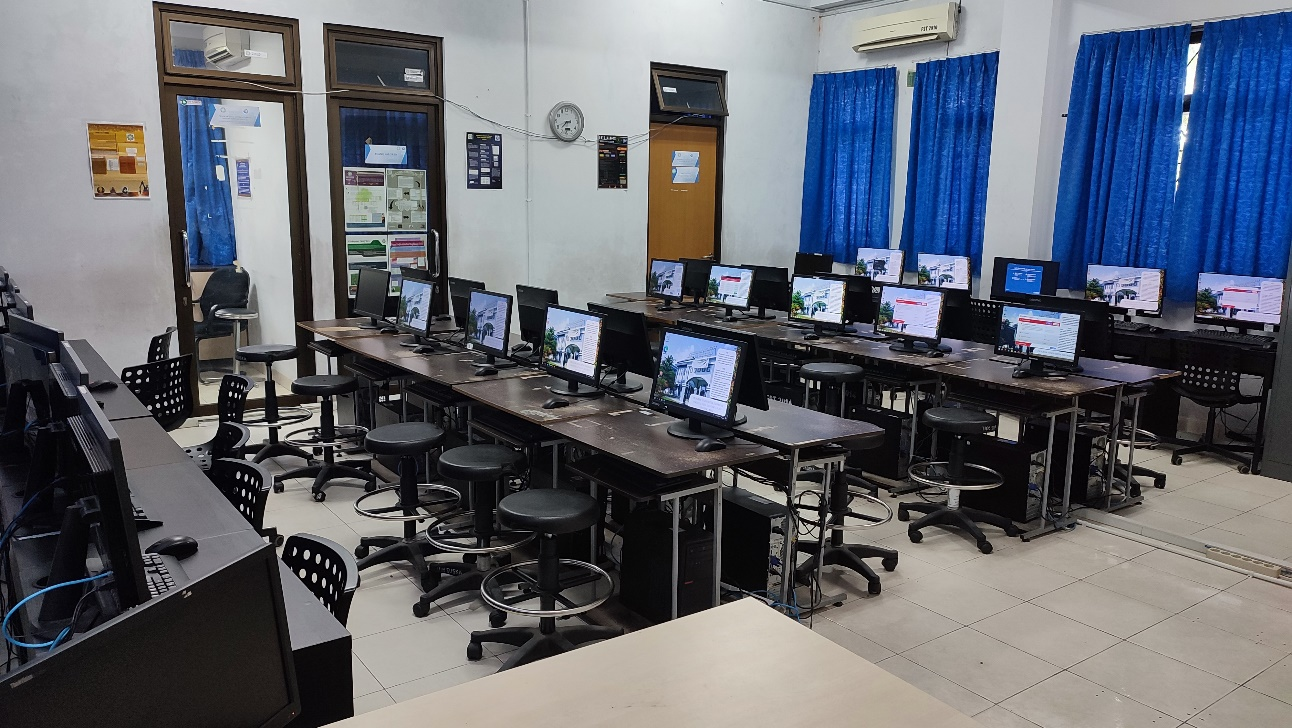
\includegraphics[width=0.82\linewidth]{konten/gambar/lab-rsi.jpg}
	\caption{Laboratorium Rekayasa Sistem Informasi}
	\label{fig:lab-rsi-bab2}
\end{figure}

\begin{figure}
	\centering
	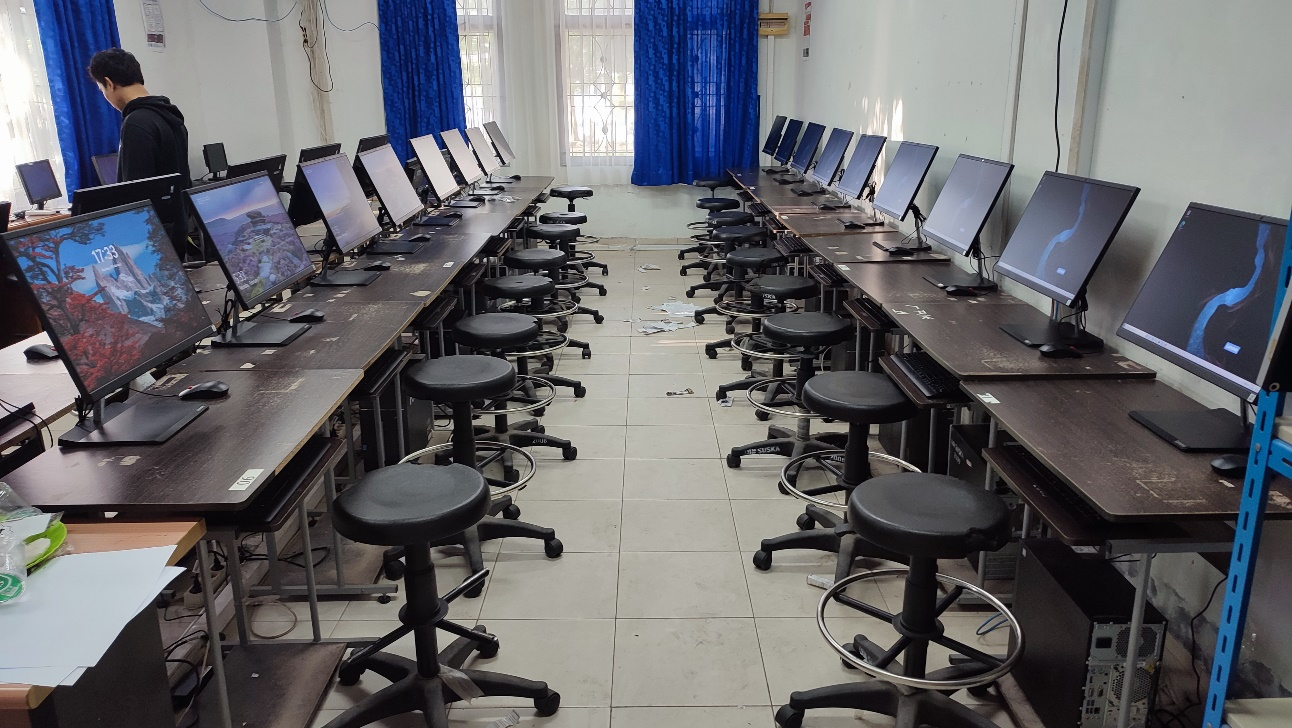
\includegraphics[width=0.82\linewidth]{konten/gambar/lab-internet.jpg}
	\caption{Laboratorium Internet}
	\label{fig:lab-int-bab2}
\end{figure}

\begin{figure}
	\centering
	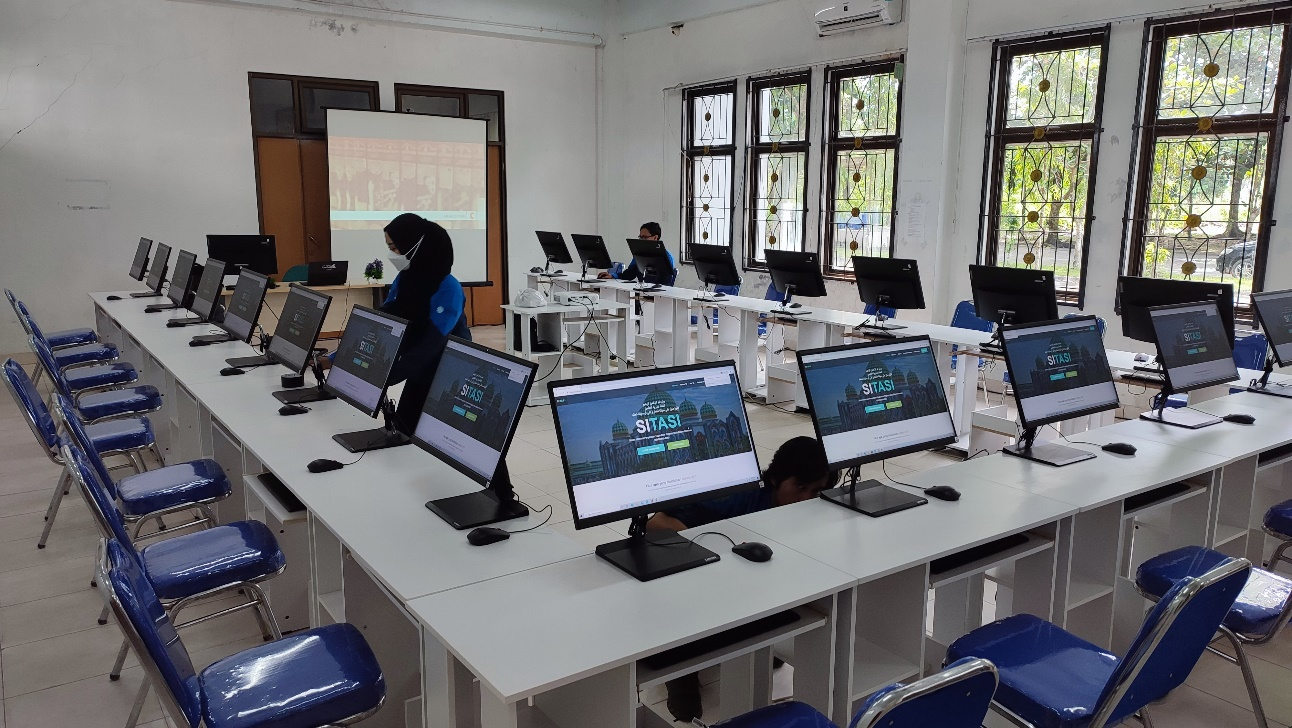
\includegraphics[width=0.82\linewidth]{konten/gambar/lab-se.jpg}
	\caption{Laboratorium \textit{Software Engineering}}
	\label{fig:lab-se-bab2}
\end{figure}

\begin{figure}
	\centering
	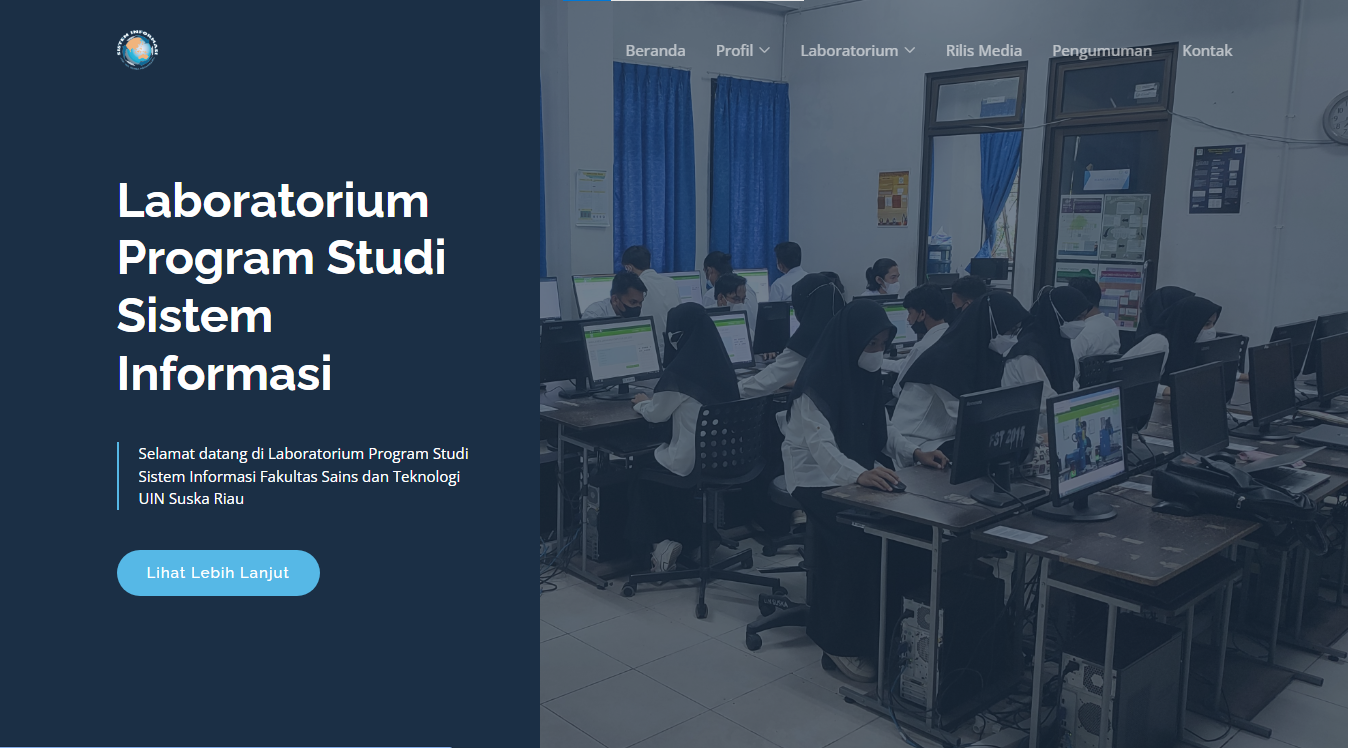
\includegraphics[width=0.82\linewidth]{konten//gambar/labsi.png}
	\caption{Website Laboratorium Program Studi Sistem Informasi}
	\label{fig:labsi-website-bab2}
\end{figure}

\begin{figure}
	\centering
	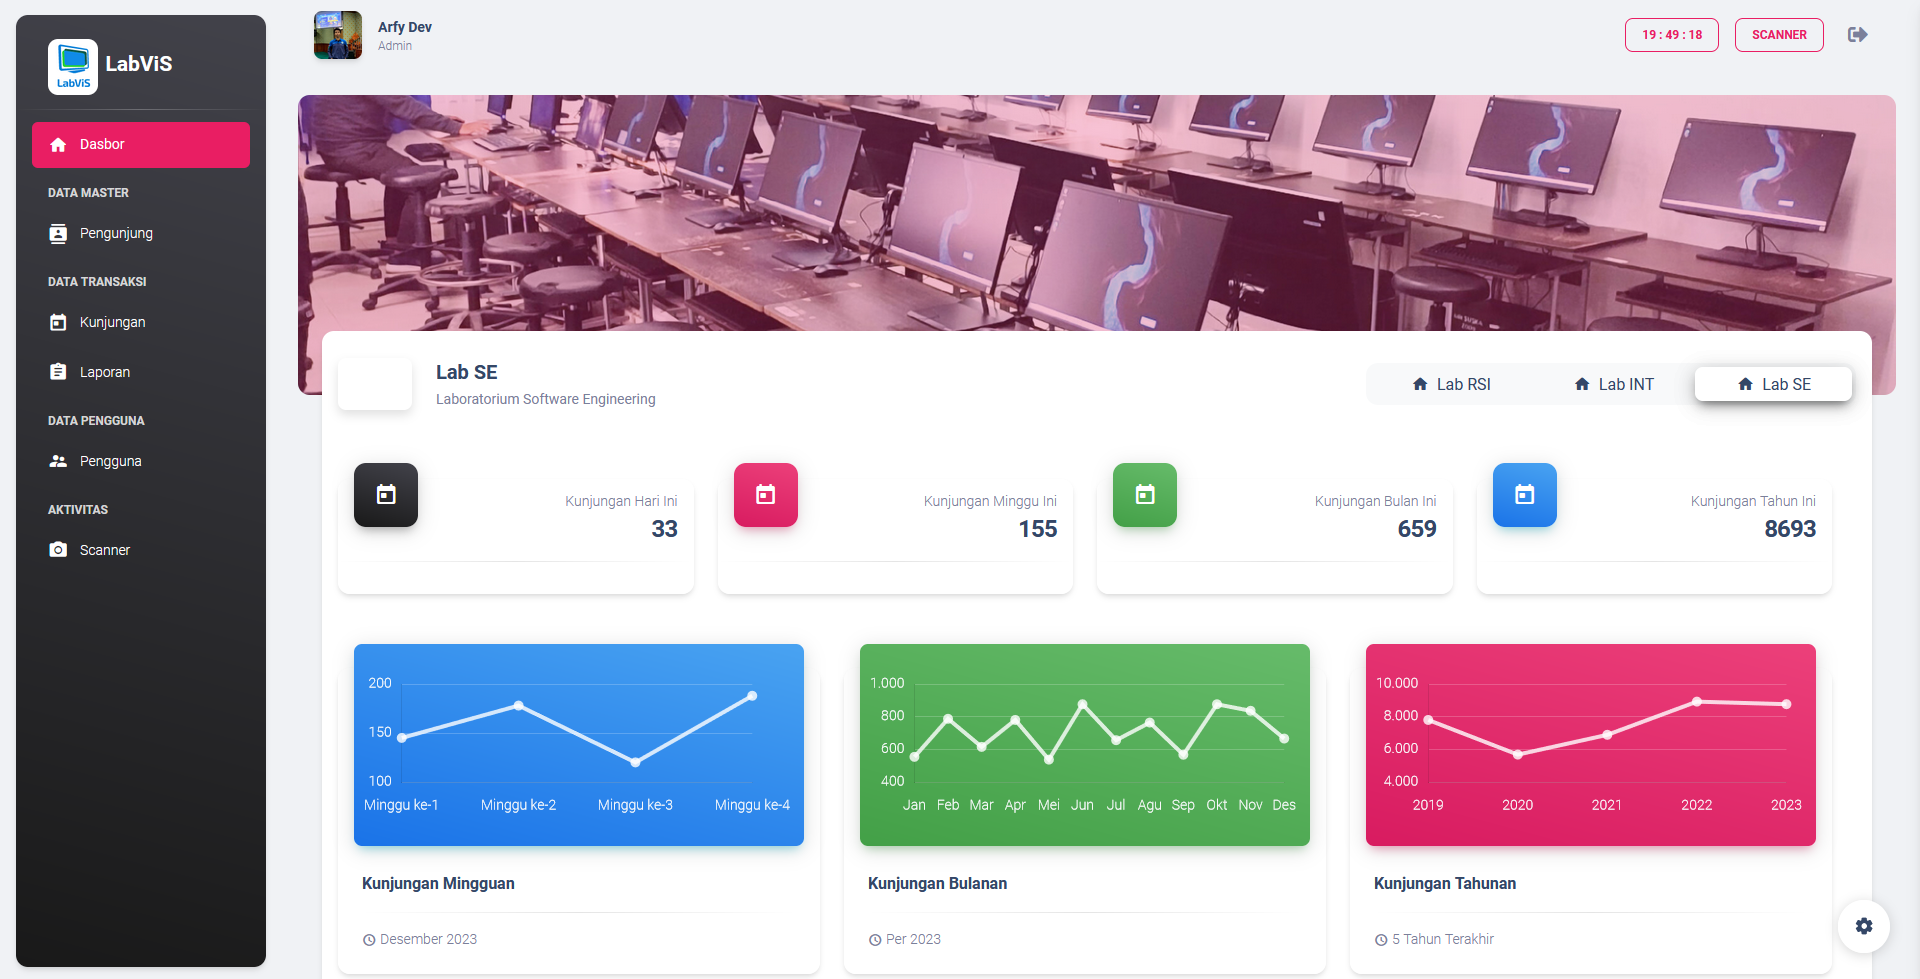
\includegraphics[width=0.82\linewidth]{konten//gambar/labvis.png}
	\caption{\textit{Laboratory Visitor System} (LABVIS)}
	\label{fig:labvis-bab2}
\end{figure}

\begin{figure}
	\centering
	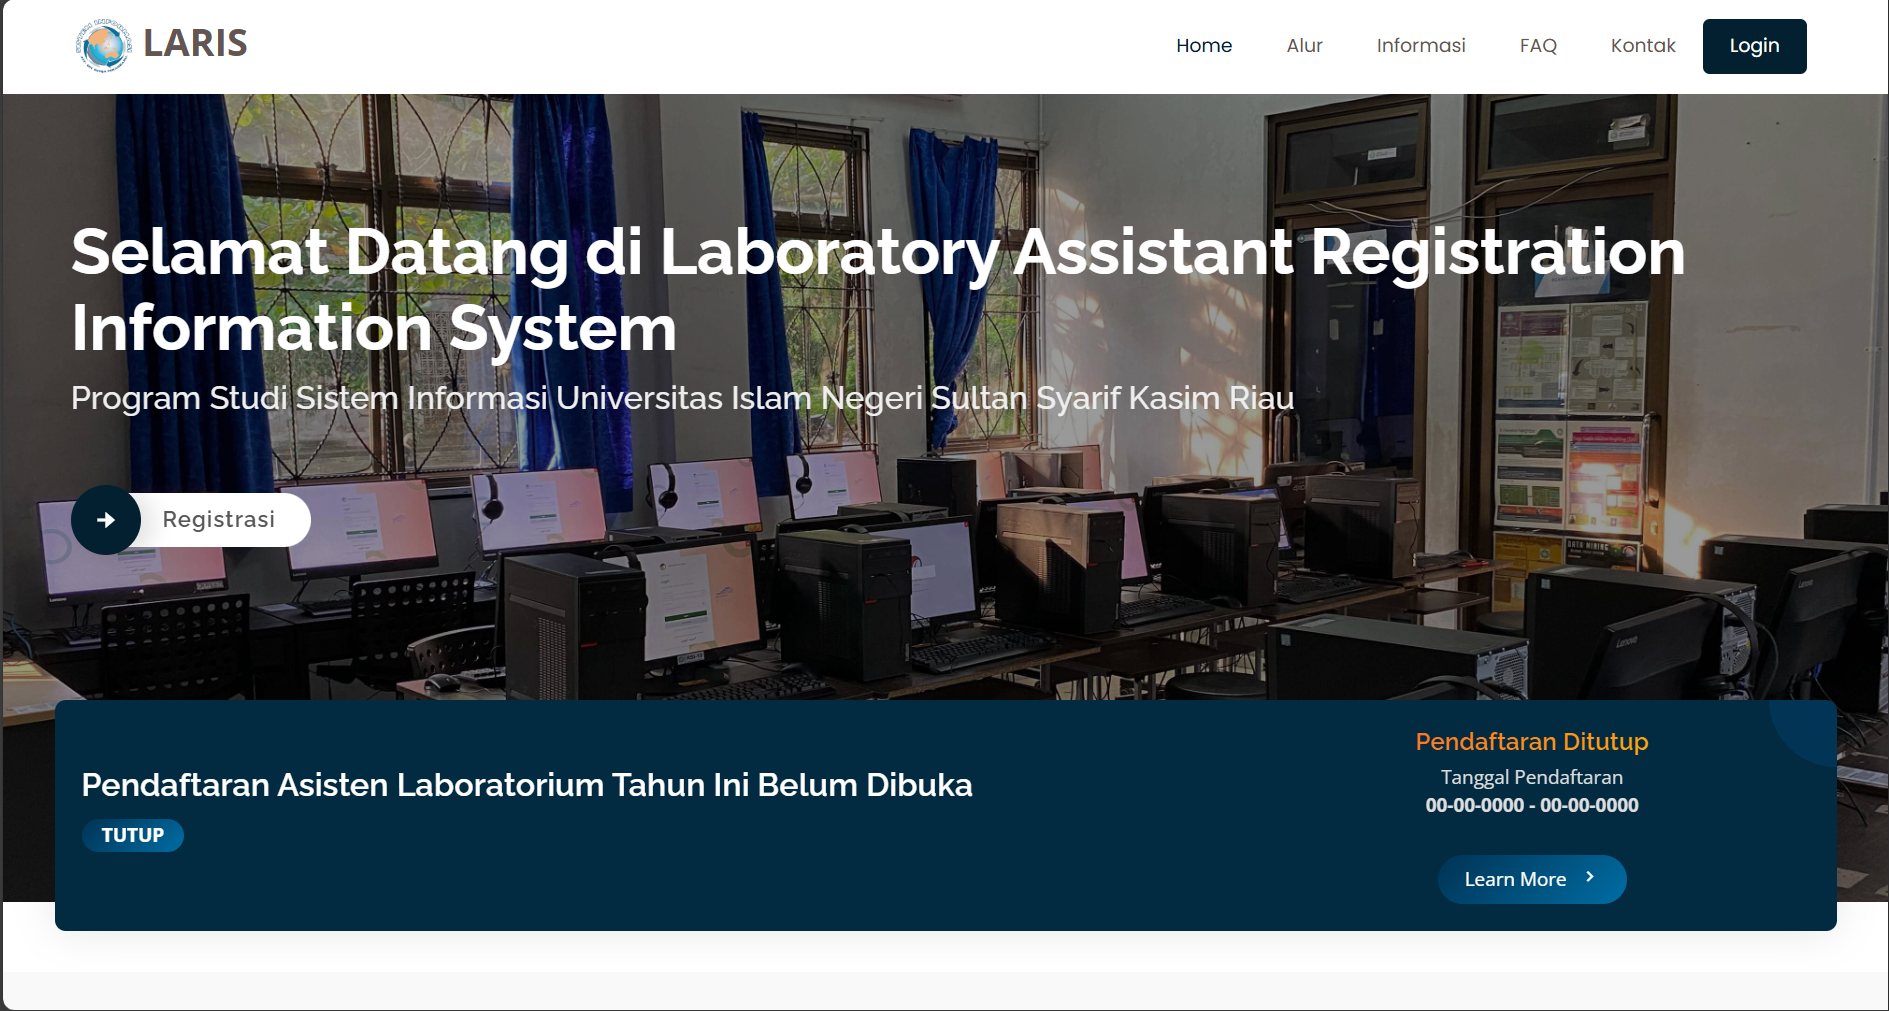
\includegraphics[width=0.82\linewidth]{konten//gambar/laris.png}
	\caption{\textit{Laboratory Assistant Registration Information System} (LARIS)}
	\label{fig:laris-bab2}
\end{figure}

% bab 4

\begin{figure}
	\centering
	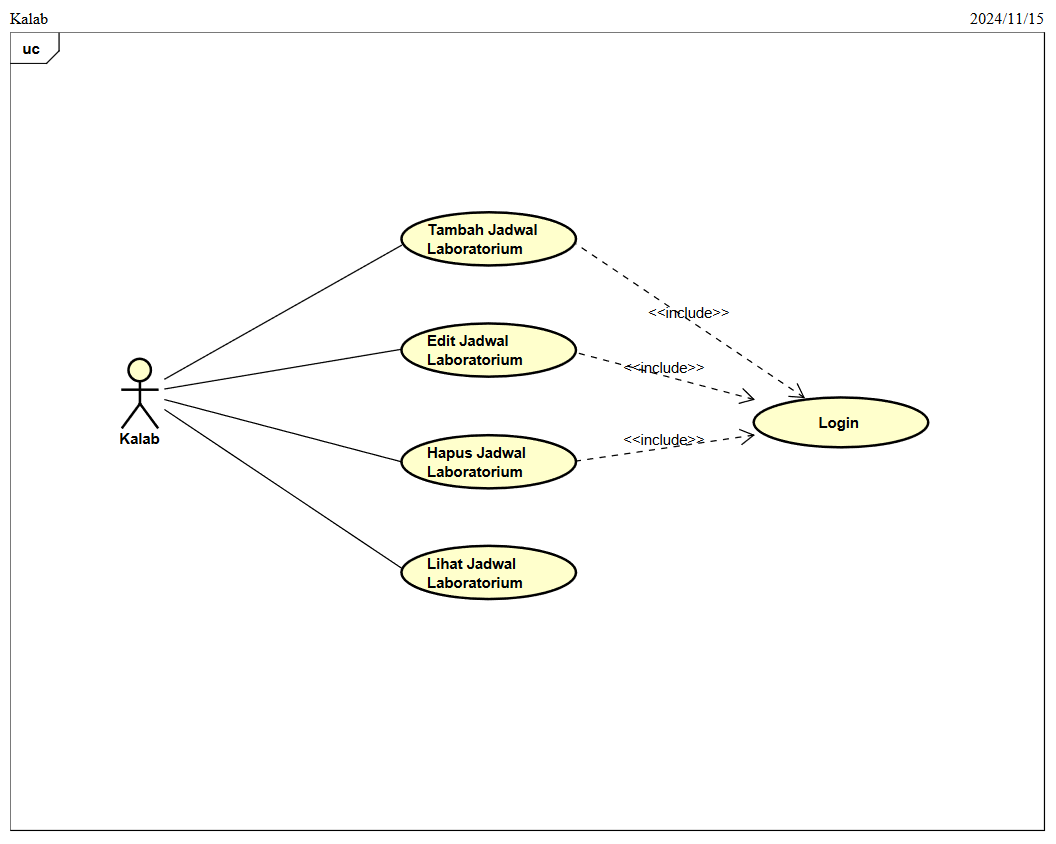
\includegraphics[width=0.82\textwidth]{konten/gambar/usecase-diagram/kalab.png}
	\caption{\textit{Usecase Diagram} Kalab}
	\label{usecase-diagram-kalab}
\end{figure}

\begin{figure}
	\centering
	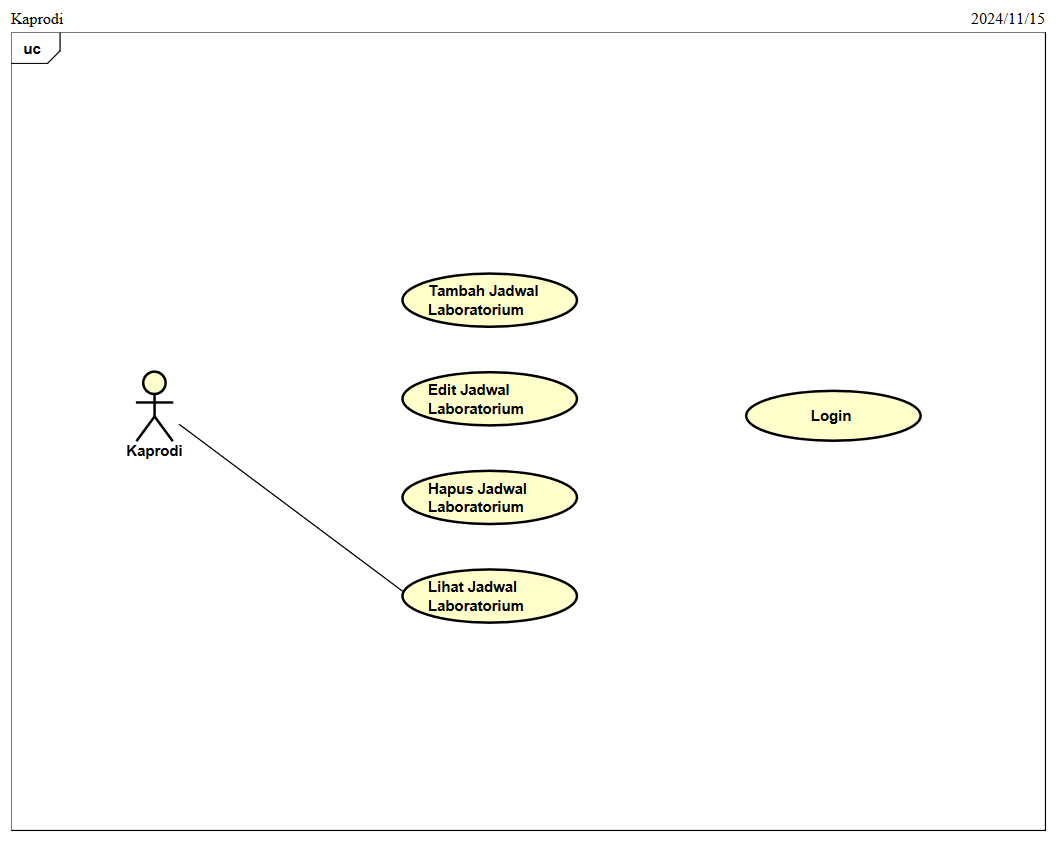
\includegraphics[width=0.82\textwidth]{konten/gambar/usecase-diagram/kaprodi.png}
	\caption{\textit{Usecase Diagram} Kaprodi}
	\label{usecase-diagram-kaprodi}
\end{figure}

\begin{figure}
	\centering
	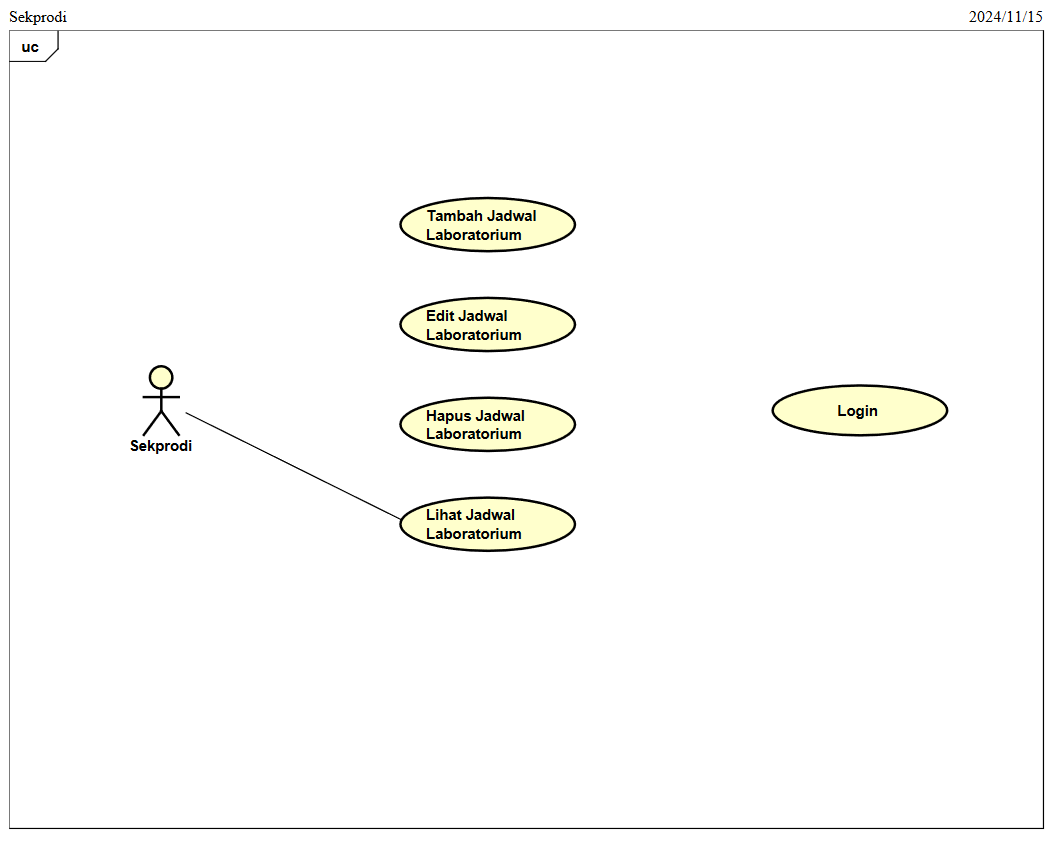
\includegraphics[width=0.82\textwidth]{konten/gambar/usecase-diagram/sekprodi.png}
	\caption{\textit{Usecase Diagram} Sekprodi}
	\label{usecase-diagram-sekprodi}
\end{figure}

\begin{figure}
	\centering
	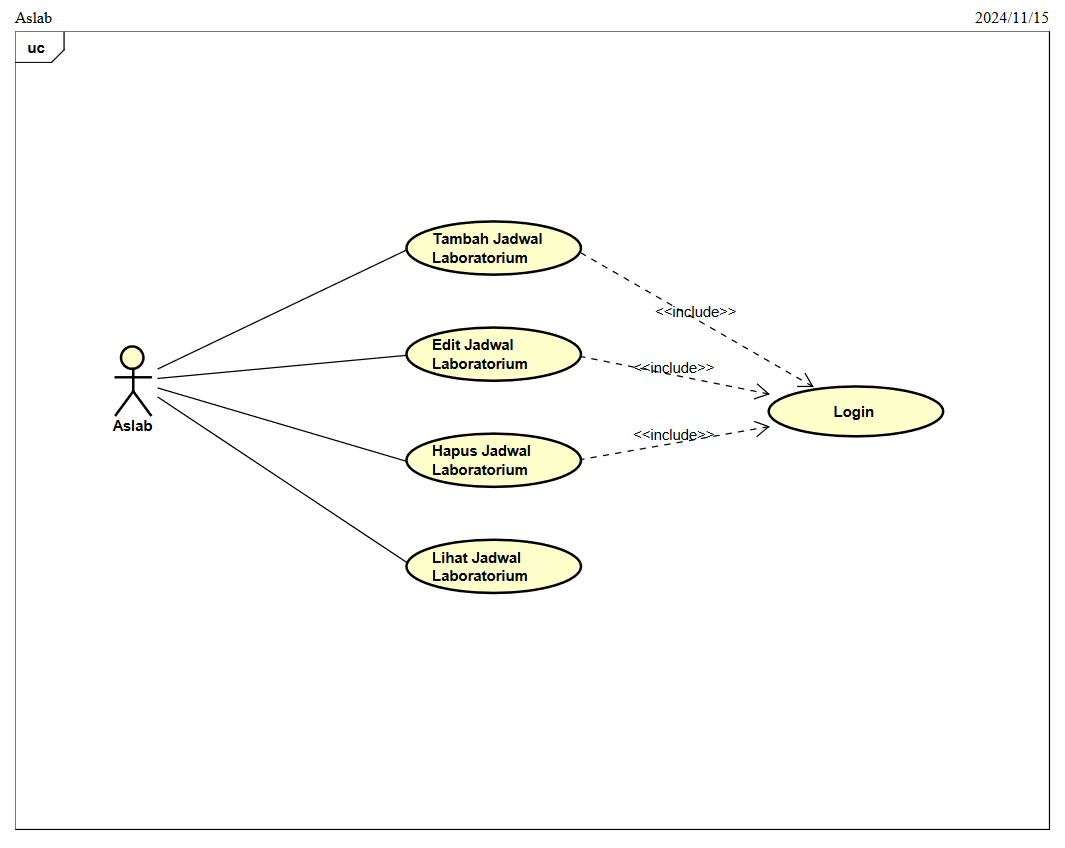
\includegraphics[width=0.82\textwidth]{konten/gambar/usecase-diagram/aslab.png}
	\caption{\textit{Usecase Diagram} Aslab}
	\label{usecase-diagram-aslab}
\end{figure}

\begin{figure}
	\centering
	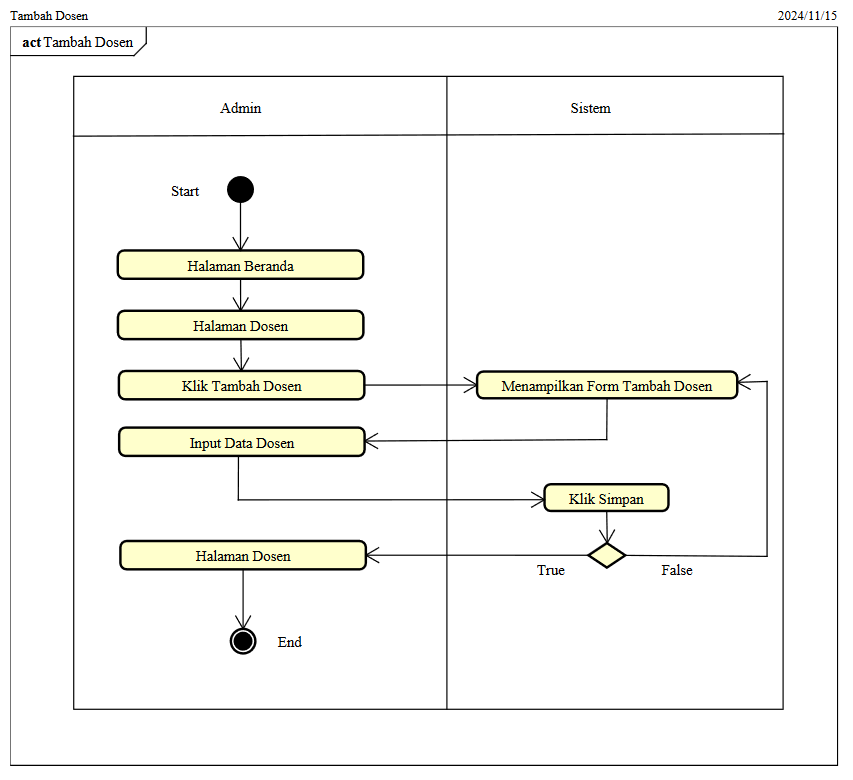
\includegraphics[width=0.82\textwidth]{konten/gambar/activity-diagram/tambah-dosen.png}
	\caption{\textit{Activity Diagram} Tambah Dosen}
	\label{activity-diagram-tambah-dosen}
\end{figure}

\begin{figure}
	\centering
	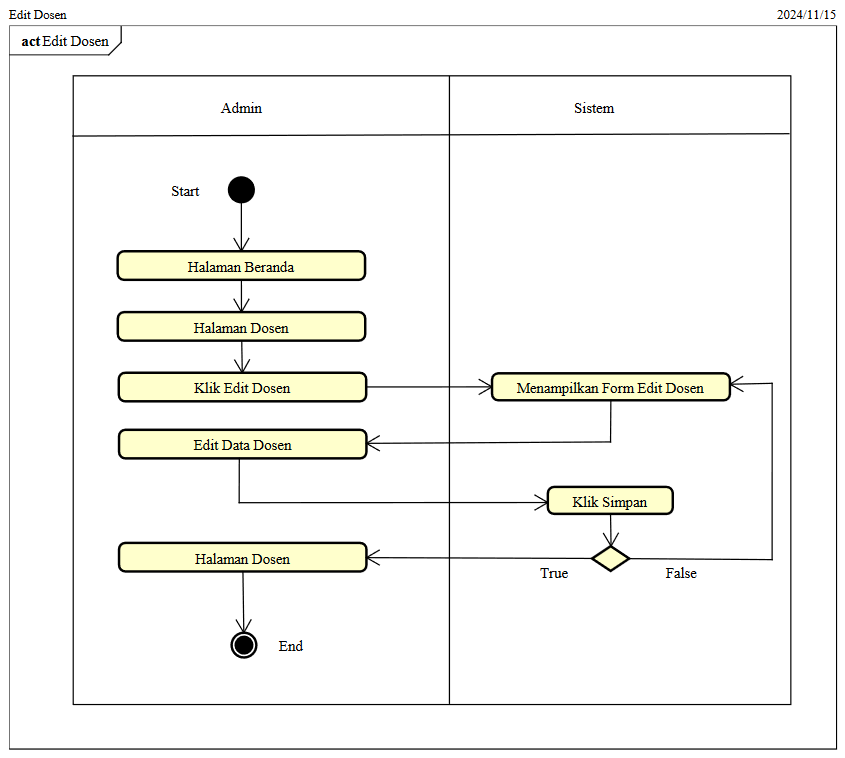
\includegraphics[width=0.82\textwidth]{konten/gambar/activity-diagram/edit-dosen.png}
	\caption{\textit{Activity Diagram} Edit Dosen}
	\label{activity-diagram-edit-dosen}
\end{figure}

\begin{figure}
	\centering
	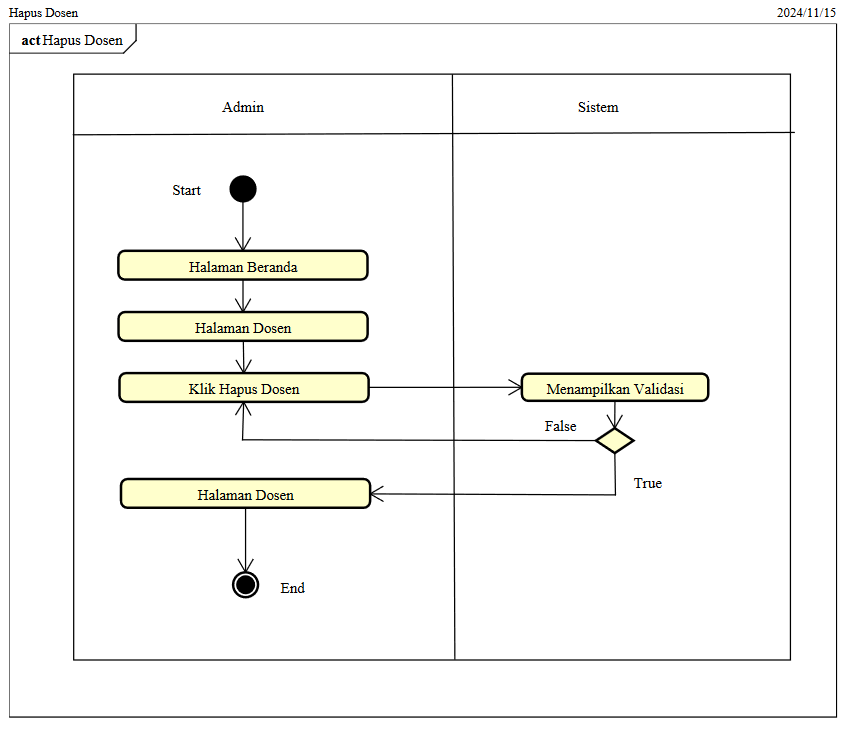
\includegraphics[width=0.82\textwidth]{konten/gambar/activity-diagram/hapus-dosen.png}
	\caption{\textit{Activity Diagram} Hapus Dosen}
	\label{activity-diagram-hapus-dosen}
\end{figure}

\begin{figure}
	\centering
	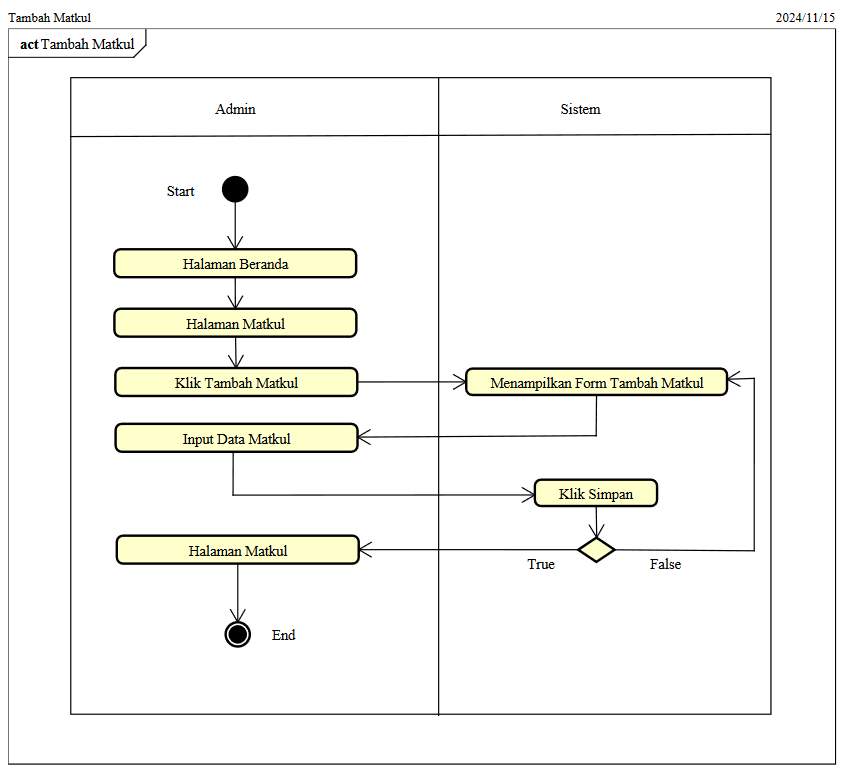
\includegraphics[width=0.82\textwidth]{konten/gambar/activity-diagram/tambah-matkul.png}
	\caption{\textit{Activity Diagram} Tambah Mata Kuliah}
	\label{activity-diagram-tambah-matkul}
\end{figure}

\begin{figure}
	\centering
	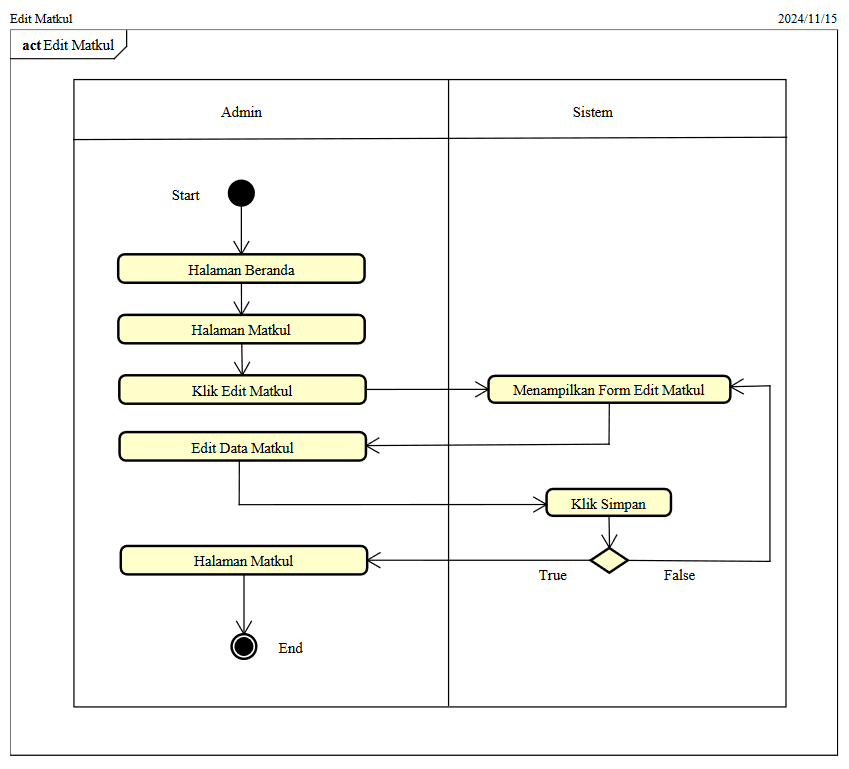
\includegraphics[width=0.82\textwidth]{konten/gambar/activity-diagram/edit-matkul.png}
	\caption{\textit{Activity Diagram} Edit Mata Kuliah}
	\label{activity-diagram-edit-matkul}
\end{figure}

\begin{figure}
	\centering
	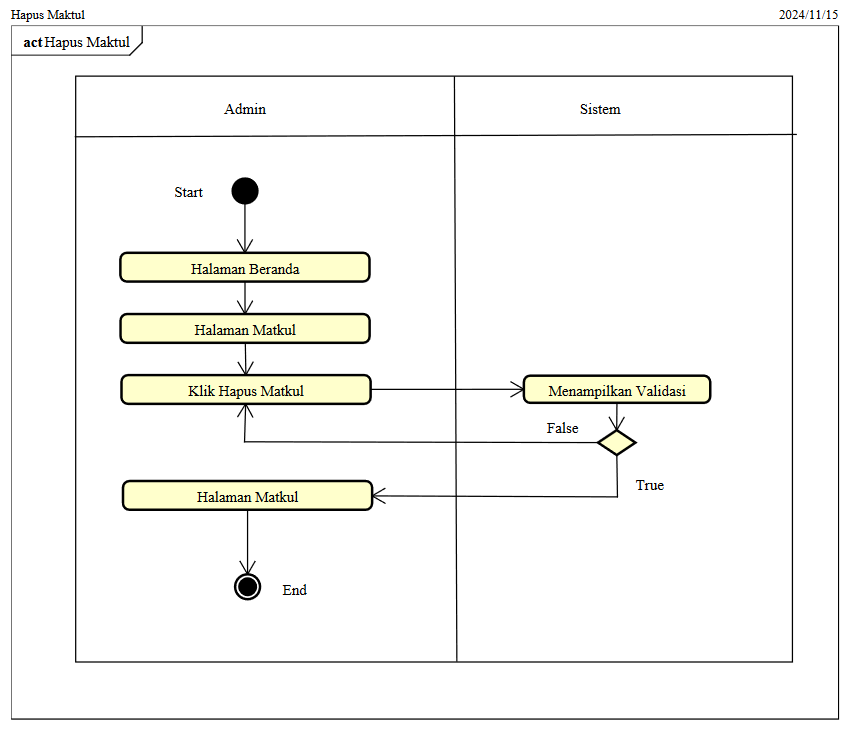
\includegraphics[width=0.82\textwidth]{konten/gambar/activity-diagram/hapus-matkul.png}
	\caption{\textit{Activity Diagram} Hapus Mata Kuliah}
	\label{activity-diagram-hapus-matkul}
\end{figure}

\begin{figure}
	\centering
	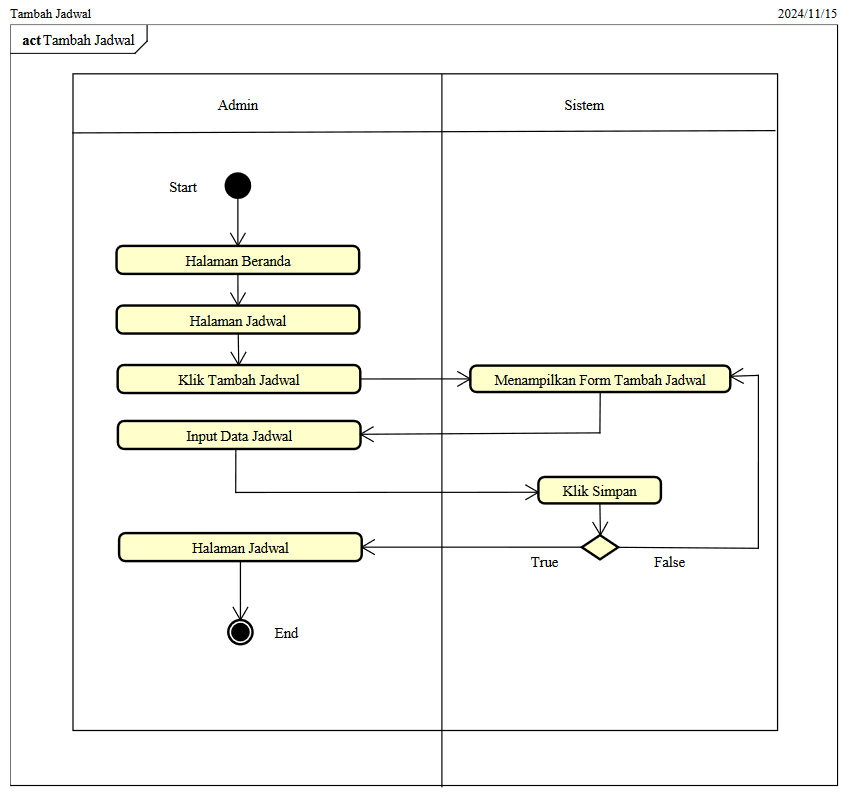
\includegraphics[width=0.82\textwidth]{konten/gambar/activity-diagram/tambah-jadwal.png}
	\caption{\textit{Activity Diagram} Tambah Jadwal}
	\label{activity-diagram-tambah-jadwal}
\end{figure}

\begin{figure}
	\centering
	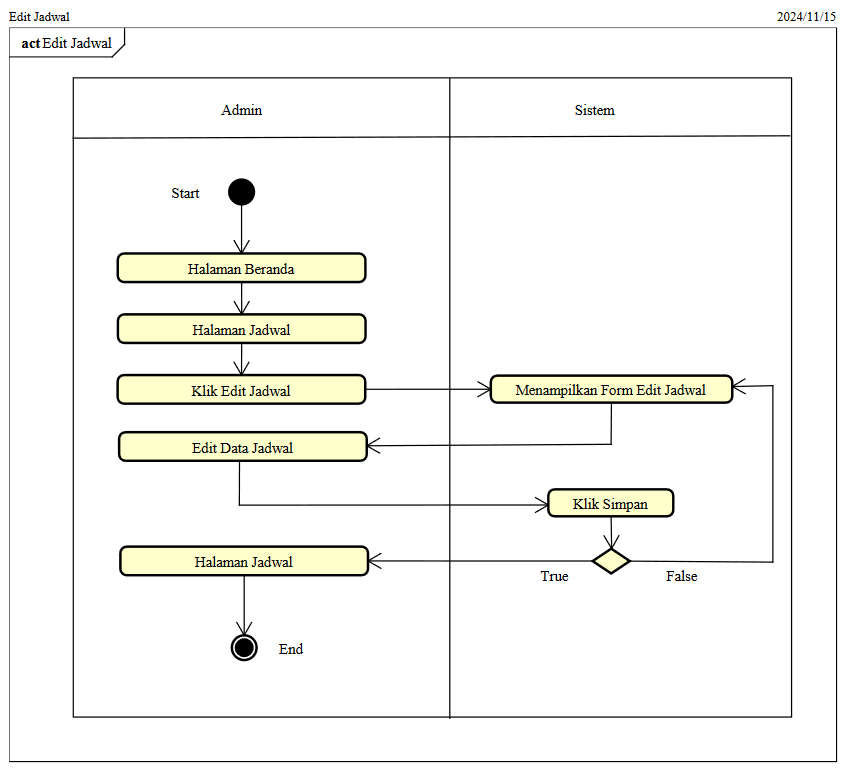
\includegraphics[width=0.82\textwidth]{konten/gambar/activity-diagram/edit-jadwal.png}
	\caption{\textit{Activity Diagram} Edit Jadwal}
	\label{activity-diagram-edit-jadwal}
\end{figure}

\begin{figure}
	\centering
	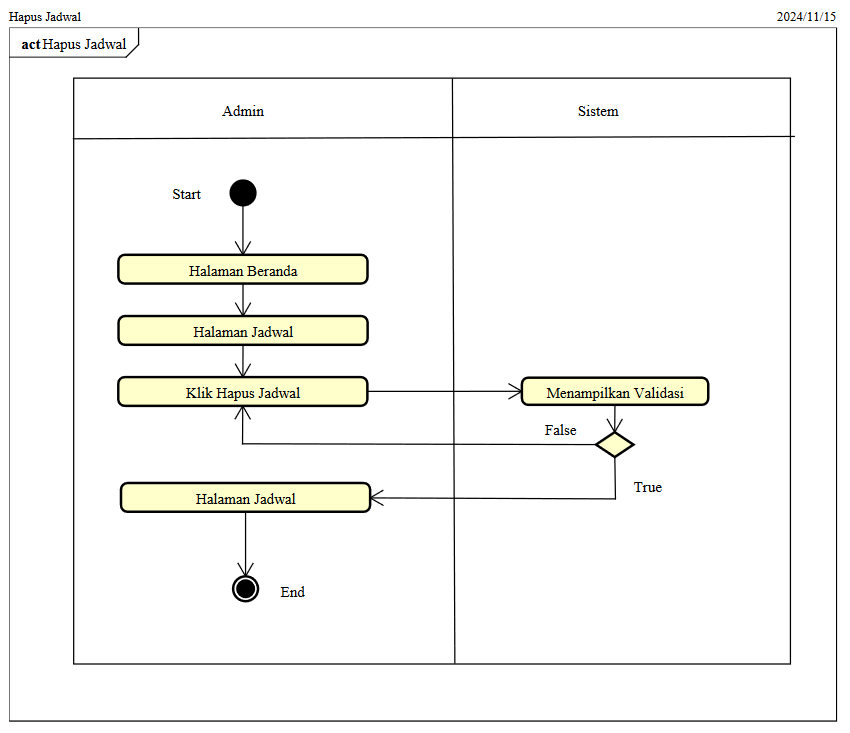
\includegraphics[width=0.82\textwidth]{konten/gambar/activity-diagram/hapus-jadwal.png}
	\caption{\textit{Activity Diagram} Hapus Jadwal}
	\label{activity-diagram-hapus-jadwal}
\end{figure}

\begin{figure}
	\centering
	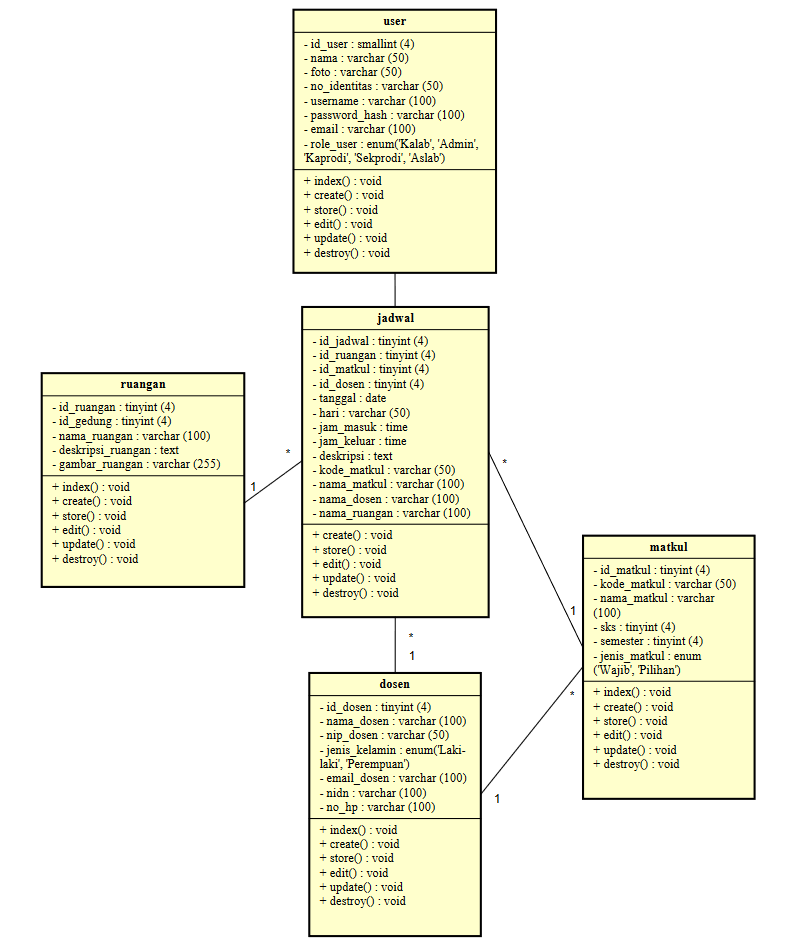
\includegraphics[width=0.82\textwidth]{konten/gambar/class-diagram.png}
	\caption{\textit{Class Diagram} ILMIS}
	\label{class-diagram}
\end{figure}

\begin{figure}
	\centering
	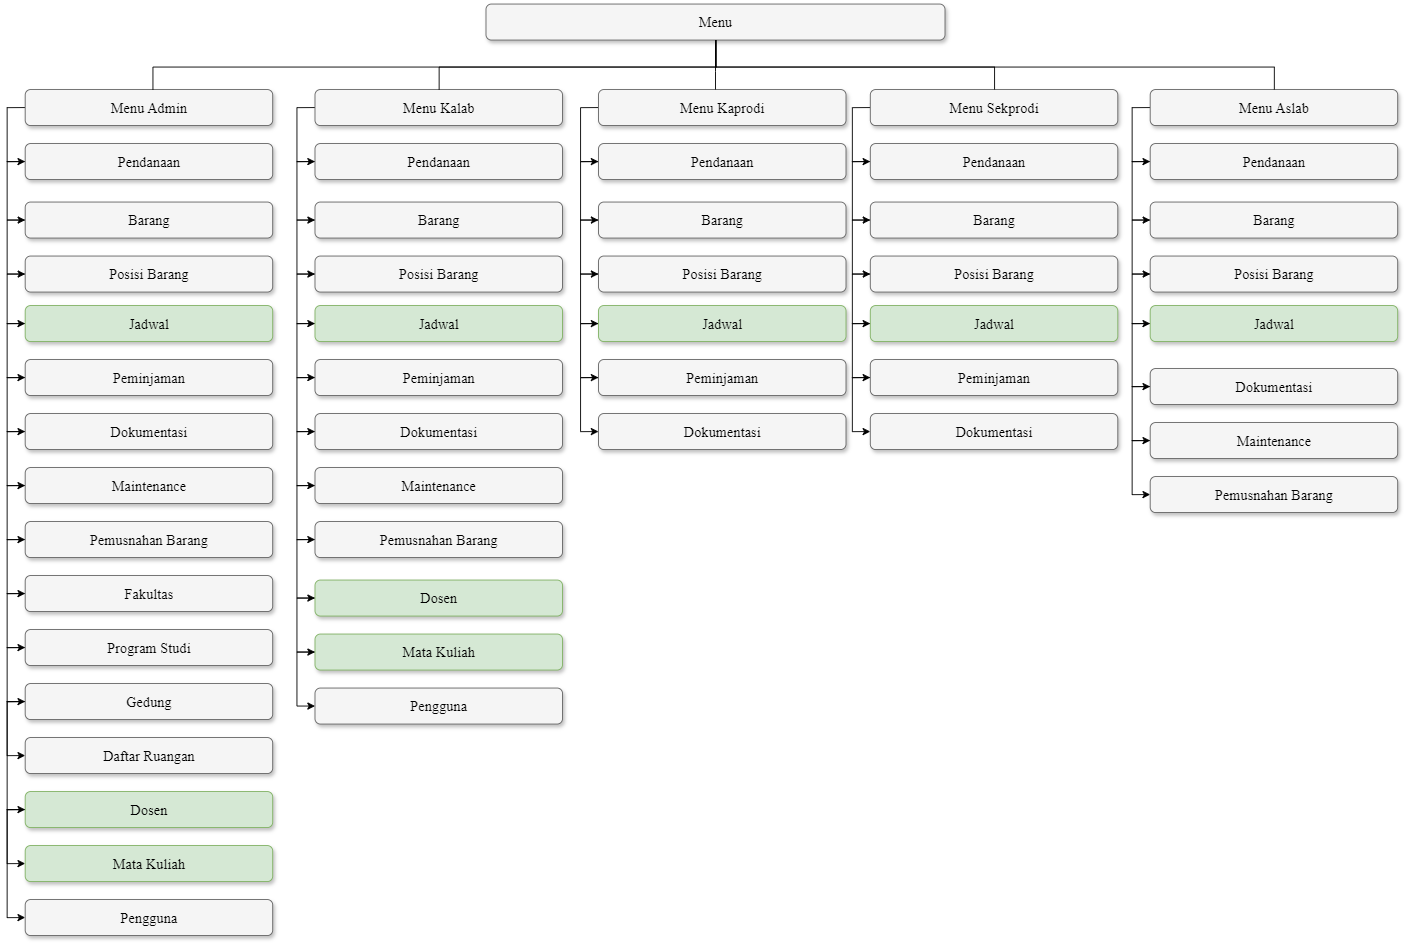
\includegraphics[width=1\textwidth]{konten/gambar/menu.png}
	\caption{Struktur Menu ILMIS}
	\label{StrukturMenuILMIS}
\end{figure}

\begin{figure}
	\centering
	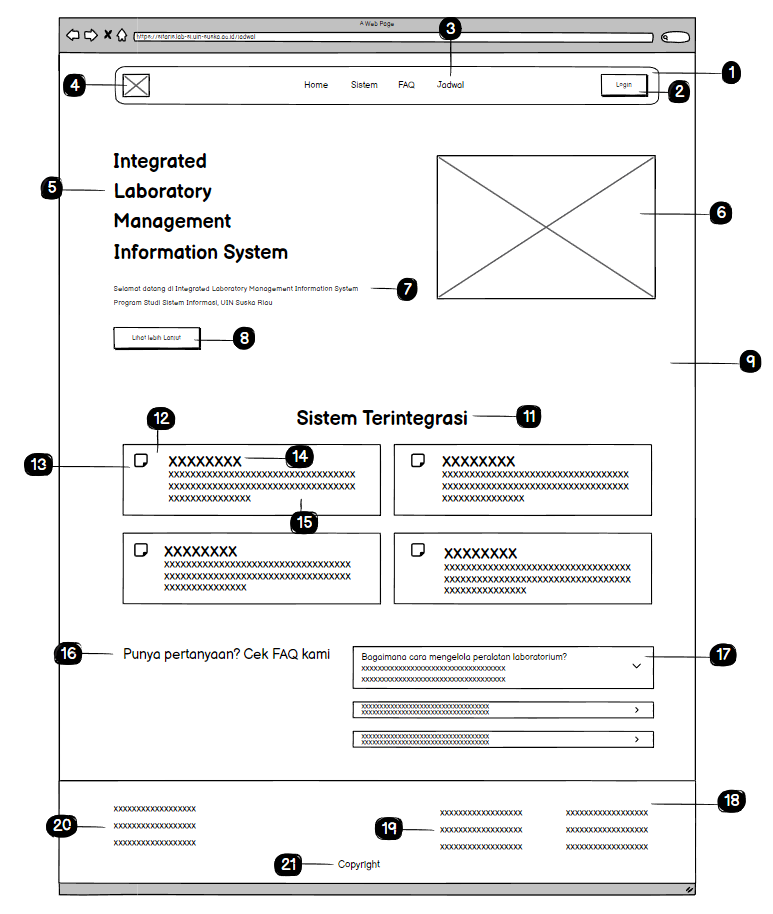
\includegraphics[width=1\textwidth]{konten/gambar/landing-page.png}
	\caption{Tampilan \textit{Landing Page} ILMIS}
	\label{fig:landing-page-interface}
\end{figure}

\begin{figure}
	\centering
	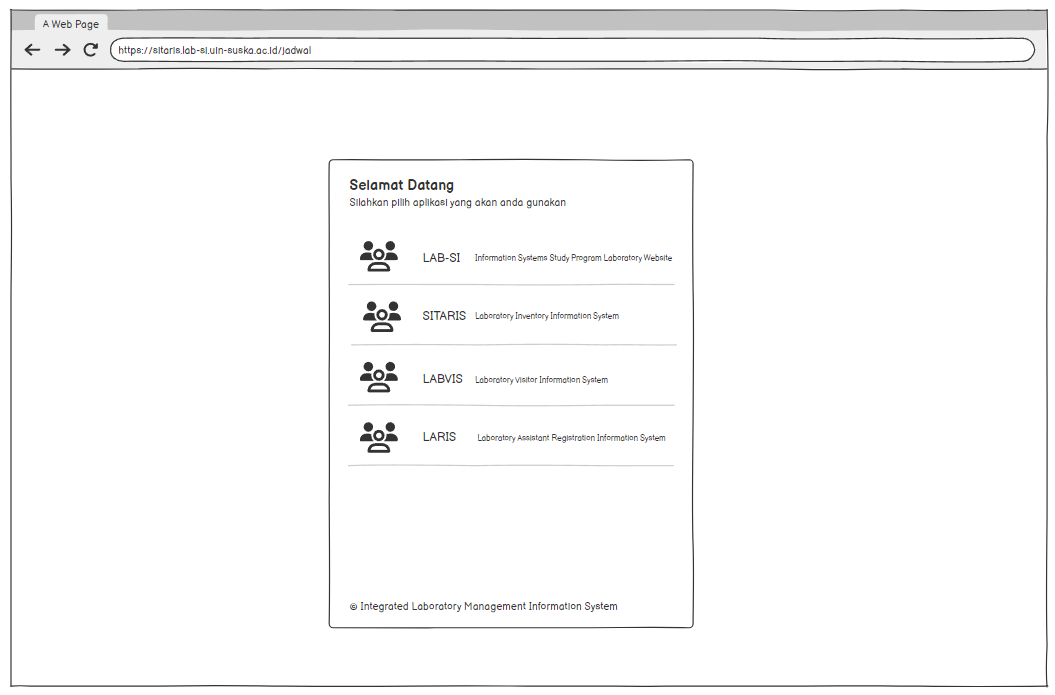
\includegraphics[width=0.82\textwidth]{konten/gambar/pilih-login.png}
	\caption{Tampilan Pilihan \textit{Login} untuk ILMIS}
	\label{fig:pilih-login-interface}
\end{figure}

\begin{figure}
	\centering
	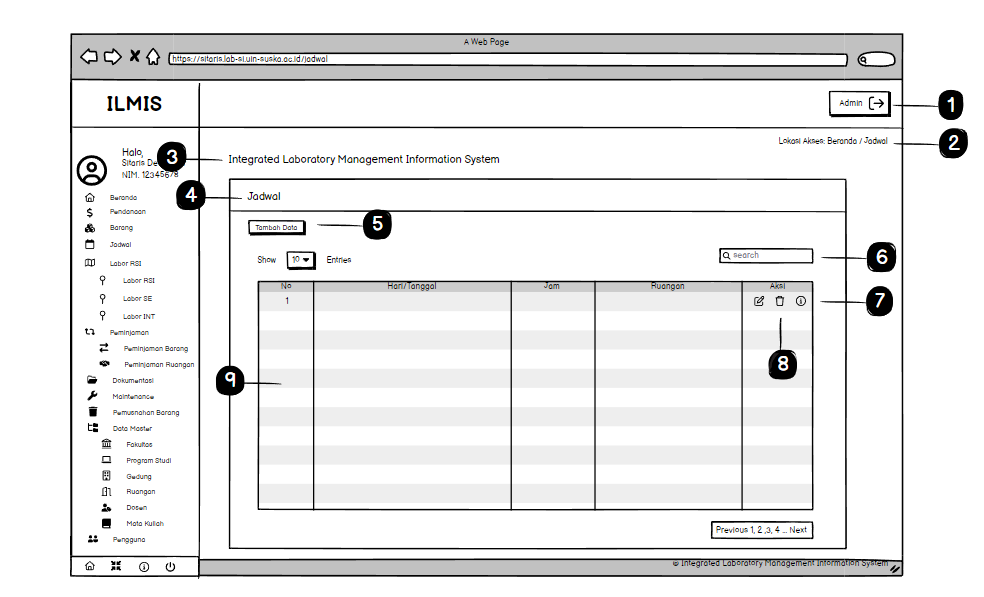
\includegraphics[width=0.92\textwidth]{konten/gambar/user interface/ui-jadwal.png}
	\caption{Tampilan Kelola Jadwal Laboratorium}
	\label{fig:kelola-jadwal}
\end{figure}

\begin{figure}
	\centering
	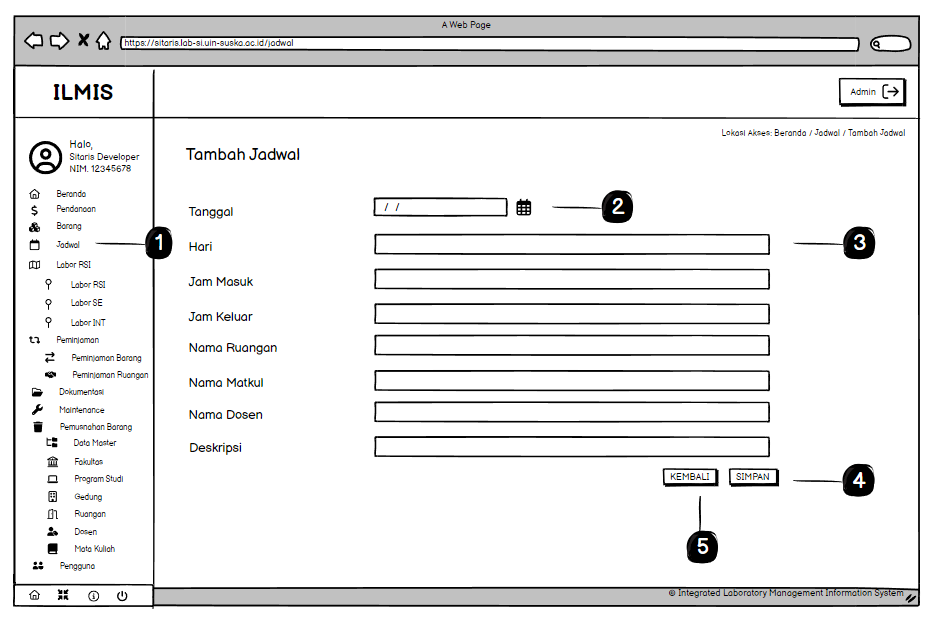
\includegraphics[width=0.82\textwidth]{konten/gambar/tambah-jadwal.png}
	\caption{Tampilan Tambah Jadwal Laboratorium}
	\label{fig:tambah-jadwal-interface}
\end{figure}

\begin{figure}
	\centering
	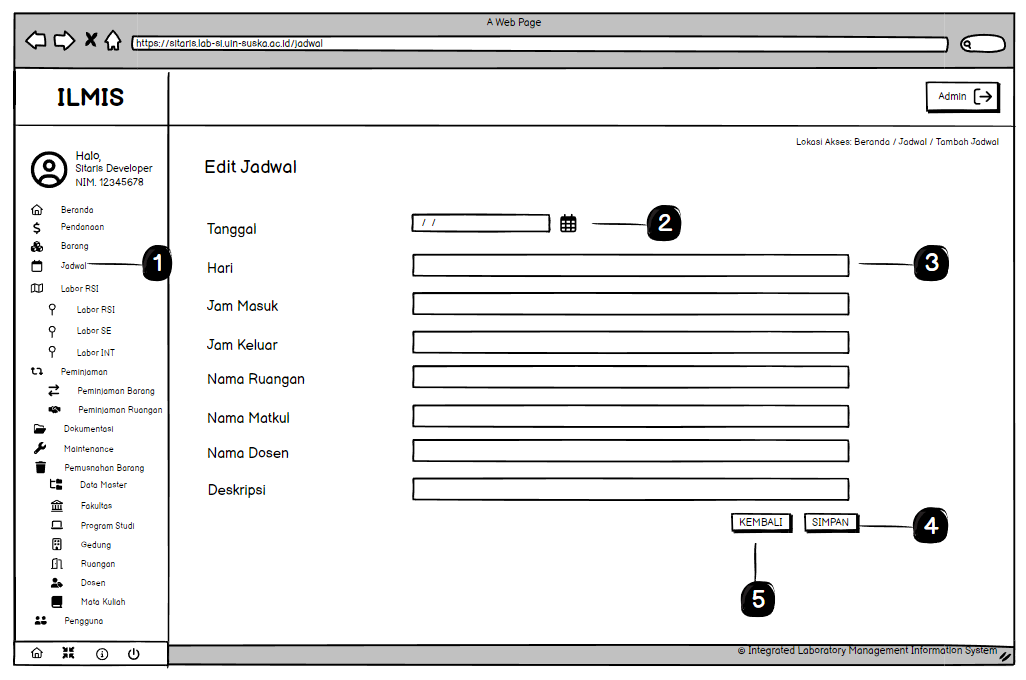
\includegraphics[width=0.82\textwidth]{konten/gambar/user interface/edit-jadwal.png}
	\caption{Tampilan Edit Jadwal Laboratorium}
	\label{fig:edit-jadwal-interface}
\end{figure}

\begin{figure}
	\centering
	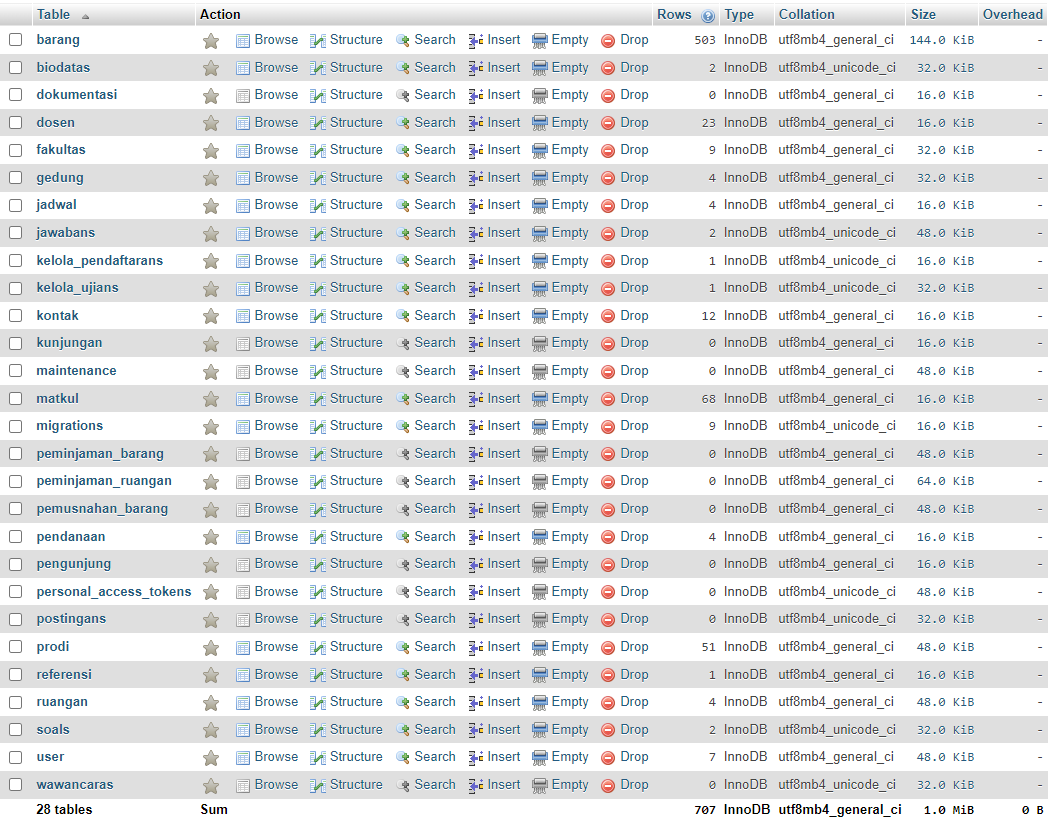
\includegraphics[width=0.82\textwidth]{konten/gambar/implementasi/database.png}
	\caption{\textit{Database}}
	\label{database-manlab}
\end{figure}

\begin{figure}
	\centering
	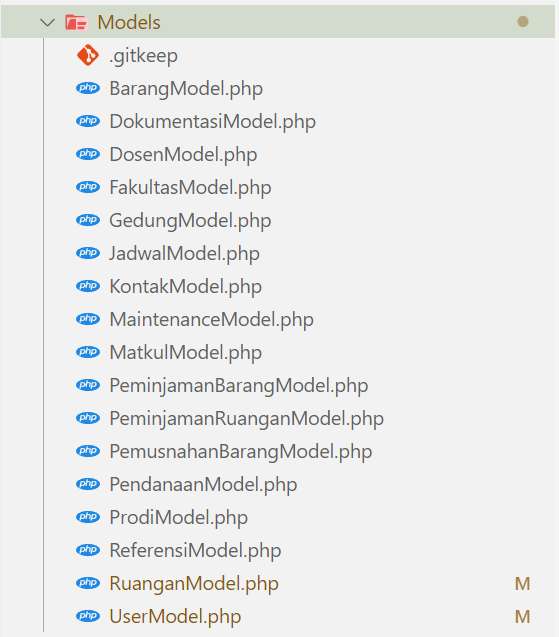
\includegraphics[width=0.82\linewidth]{konten//gambar/implementasi-folder/folder-model.png}
	\caption{Implementasi Model}
	\label{fig:implementasi-model}
\end{figure}

\begin{figure}
	\centering
	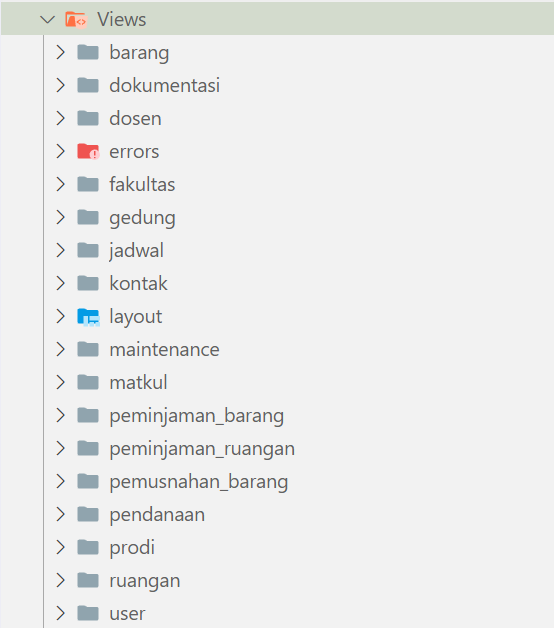
\includegraphics[width=0.82\linewidth]{konten//gambar/implementasi-folder/folder-view.png}
	\caption{Implementasi View}
	\label{fig:implementasi-view}
\end{figure}

\begin{figure}
	\centering
	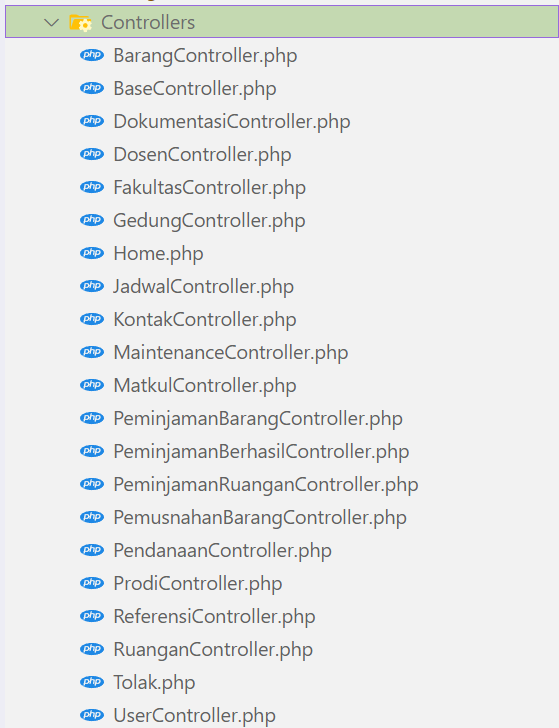
\includegraphics[width=0.82\linewidth]{konten//gambar/implementasi-folder/folder-controller.png}
	\caption{Implementasi Controller}
	\label{fig:implementasi-controller}
\end{figure}

\begin{figure}
	\centering
	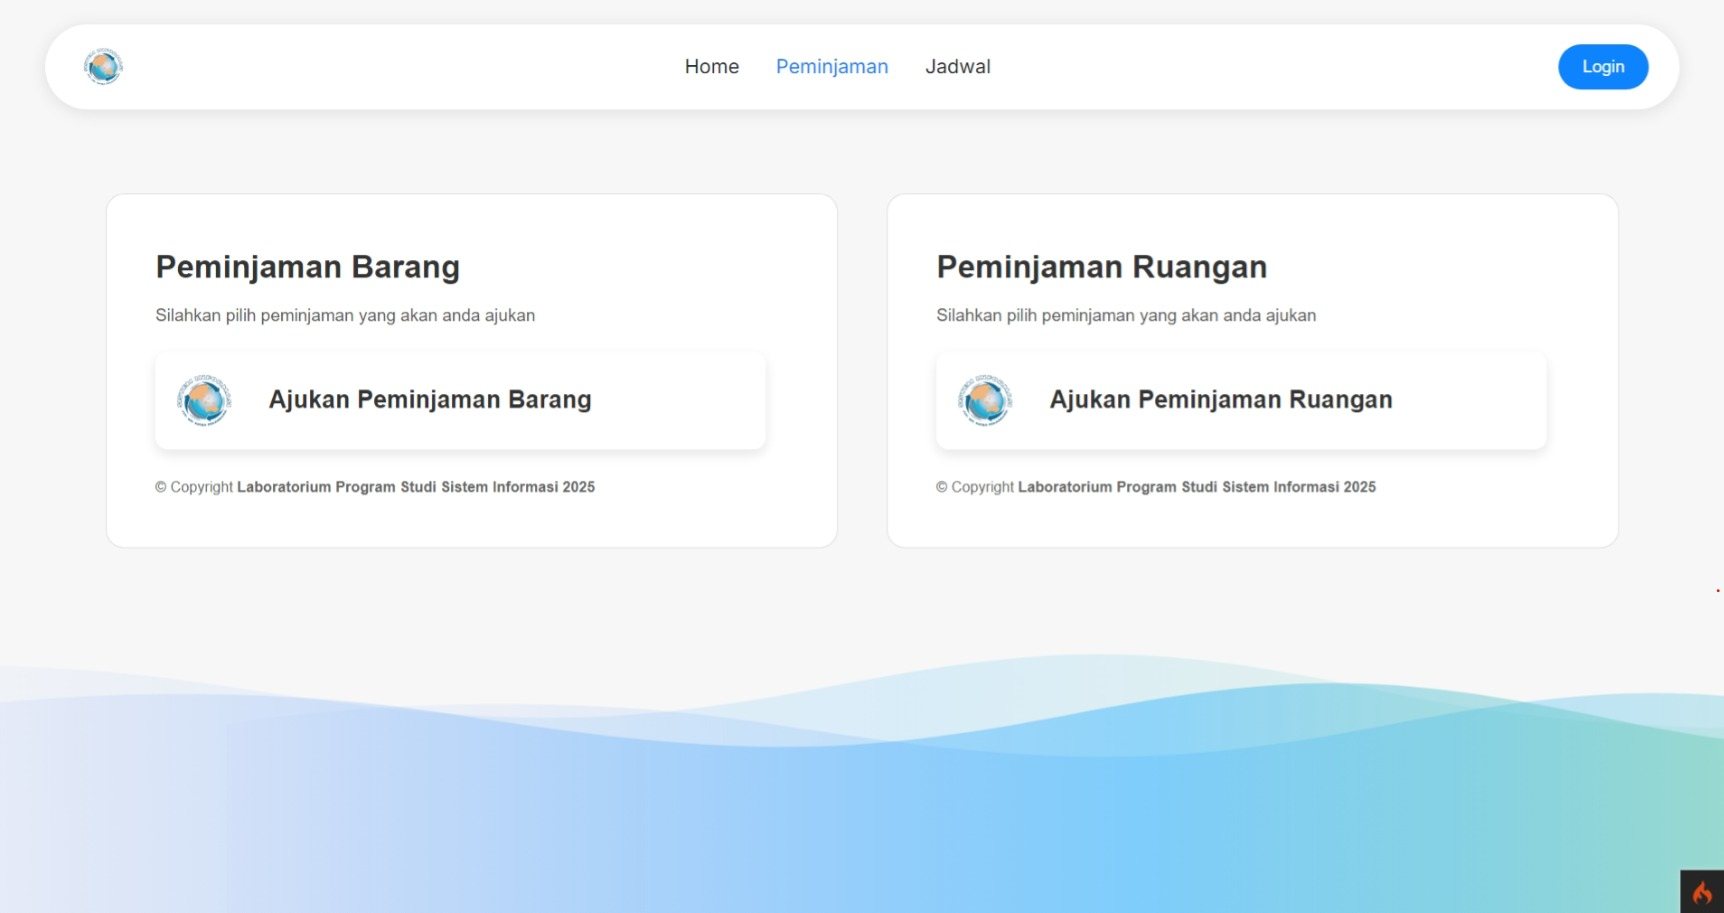
\includegraphics[width=0.82\textwidth]{konten/gambar/perbaikan/pilih-peminjaman.jpeg}
	\caption{Tampilan Pilihan Peminjaman}
	\label{fig:pilih-peminjaman}
\end{figure}

\begin{figure}
	\centering
	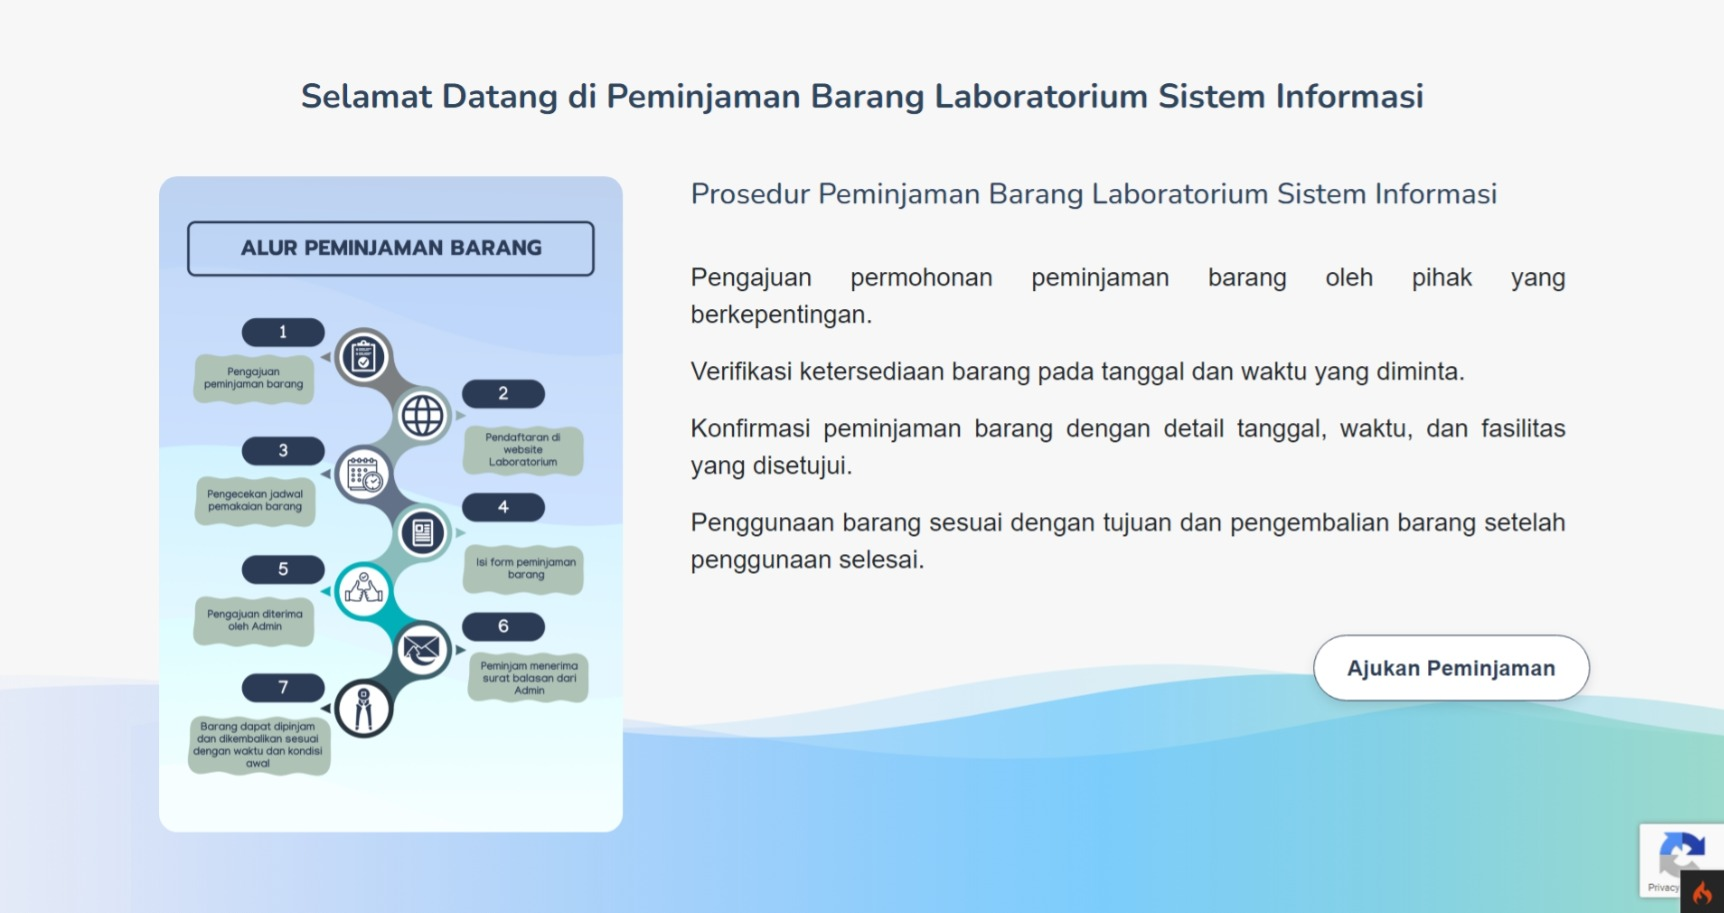
\includegraphics[width=0.82\textwidth]{konten/gambar/perbaikan/peminjaman-barang.jpeg}
	\caption{Tampilan Pengelolaan Peminjaman Barang}
	\label{fig:peminjaman-barang}
\end{figure}

\begin{figure}
	\centering
	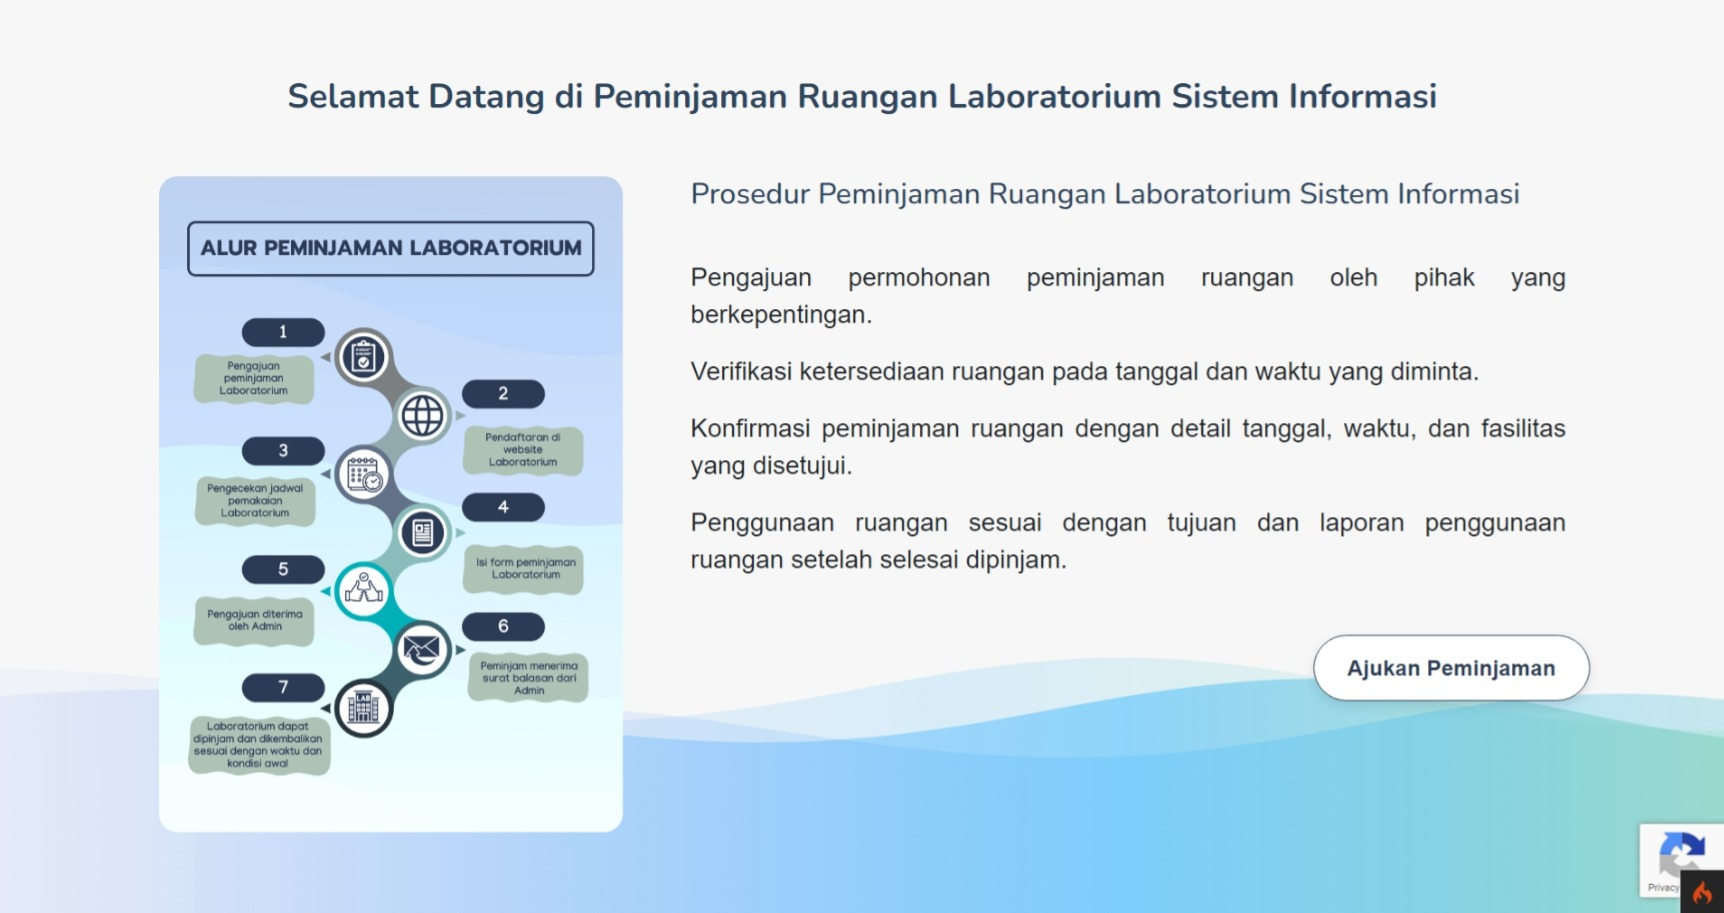
\includegraphics[width=0.82\textwidth]{konten/gambar/perbaikan/peminjaman-ruangan.jpeg}
	\caption{Tampilan Pengelolaan Peminjaman Ruangan}
	\label{fig:peminjaman-ruangan}
\end{figure}

\begin{figure}
	\centering
	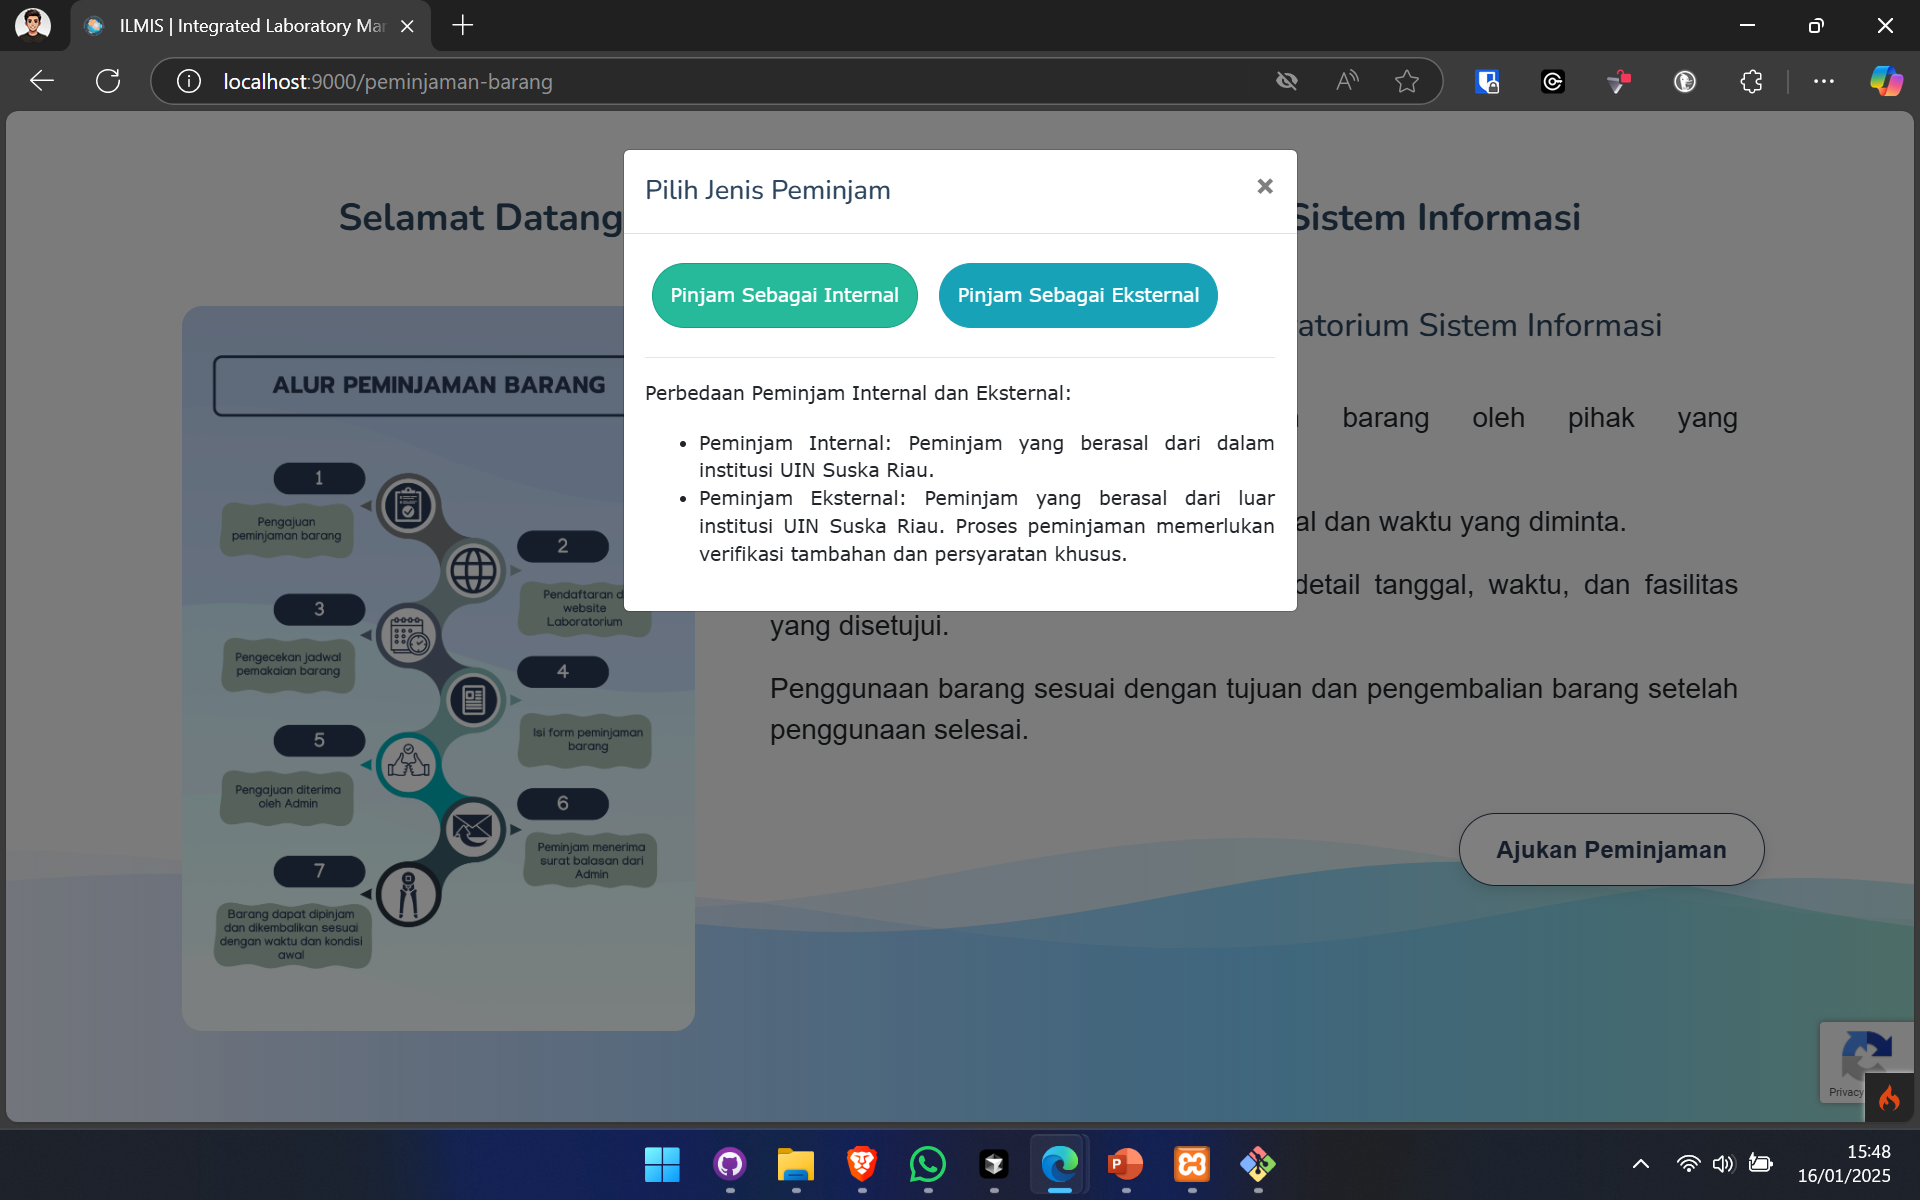
\includegraphics[width=0.82\textwidth]{konten/gambar/perbaikan/pilih-peminjam.png}
	\caption{Tampilan Pilih Peminjam}
	\label{fig:pilih-peminjam}
\end{figure}

\begin{figure}
	\centering
	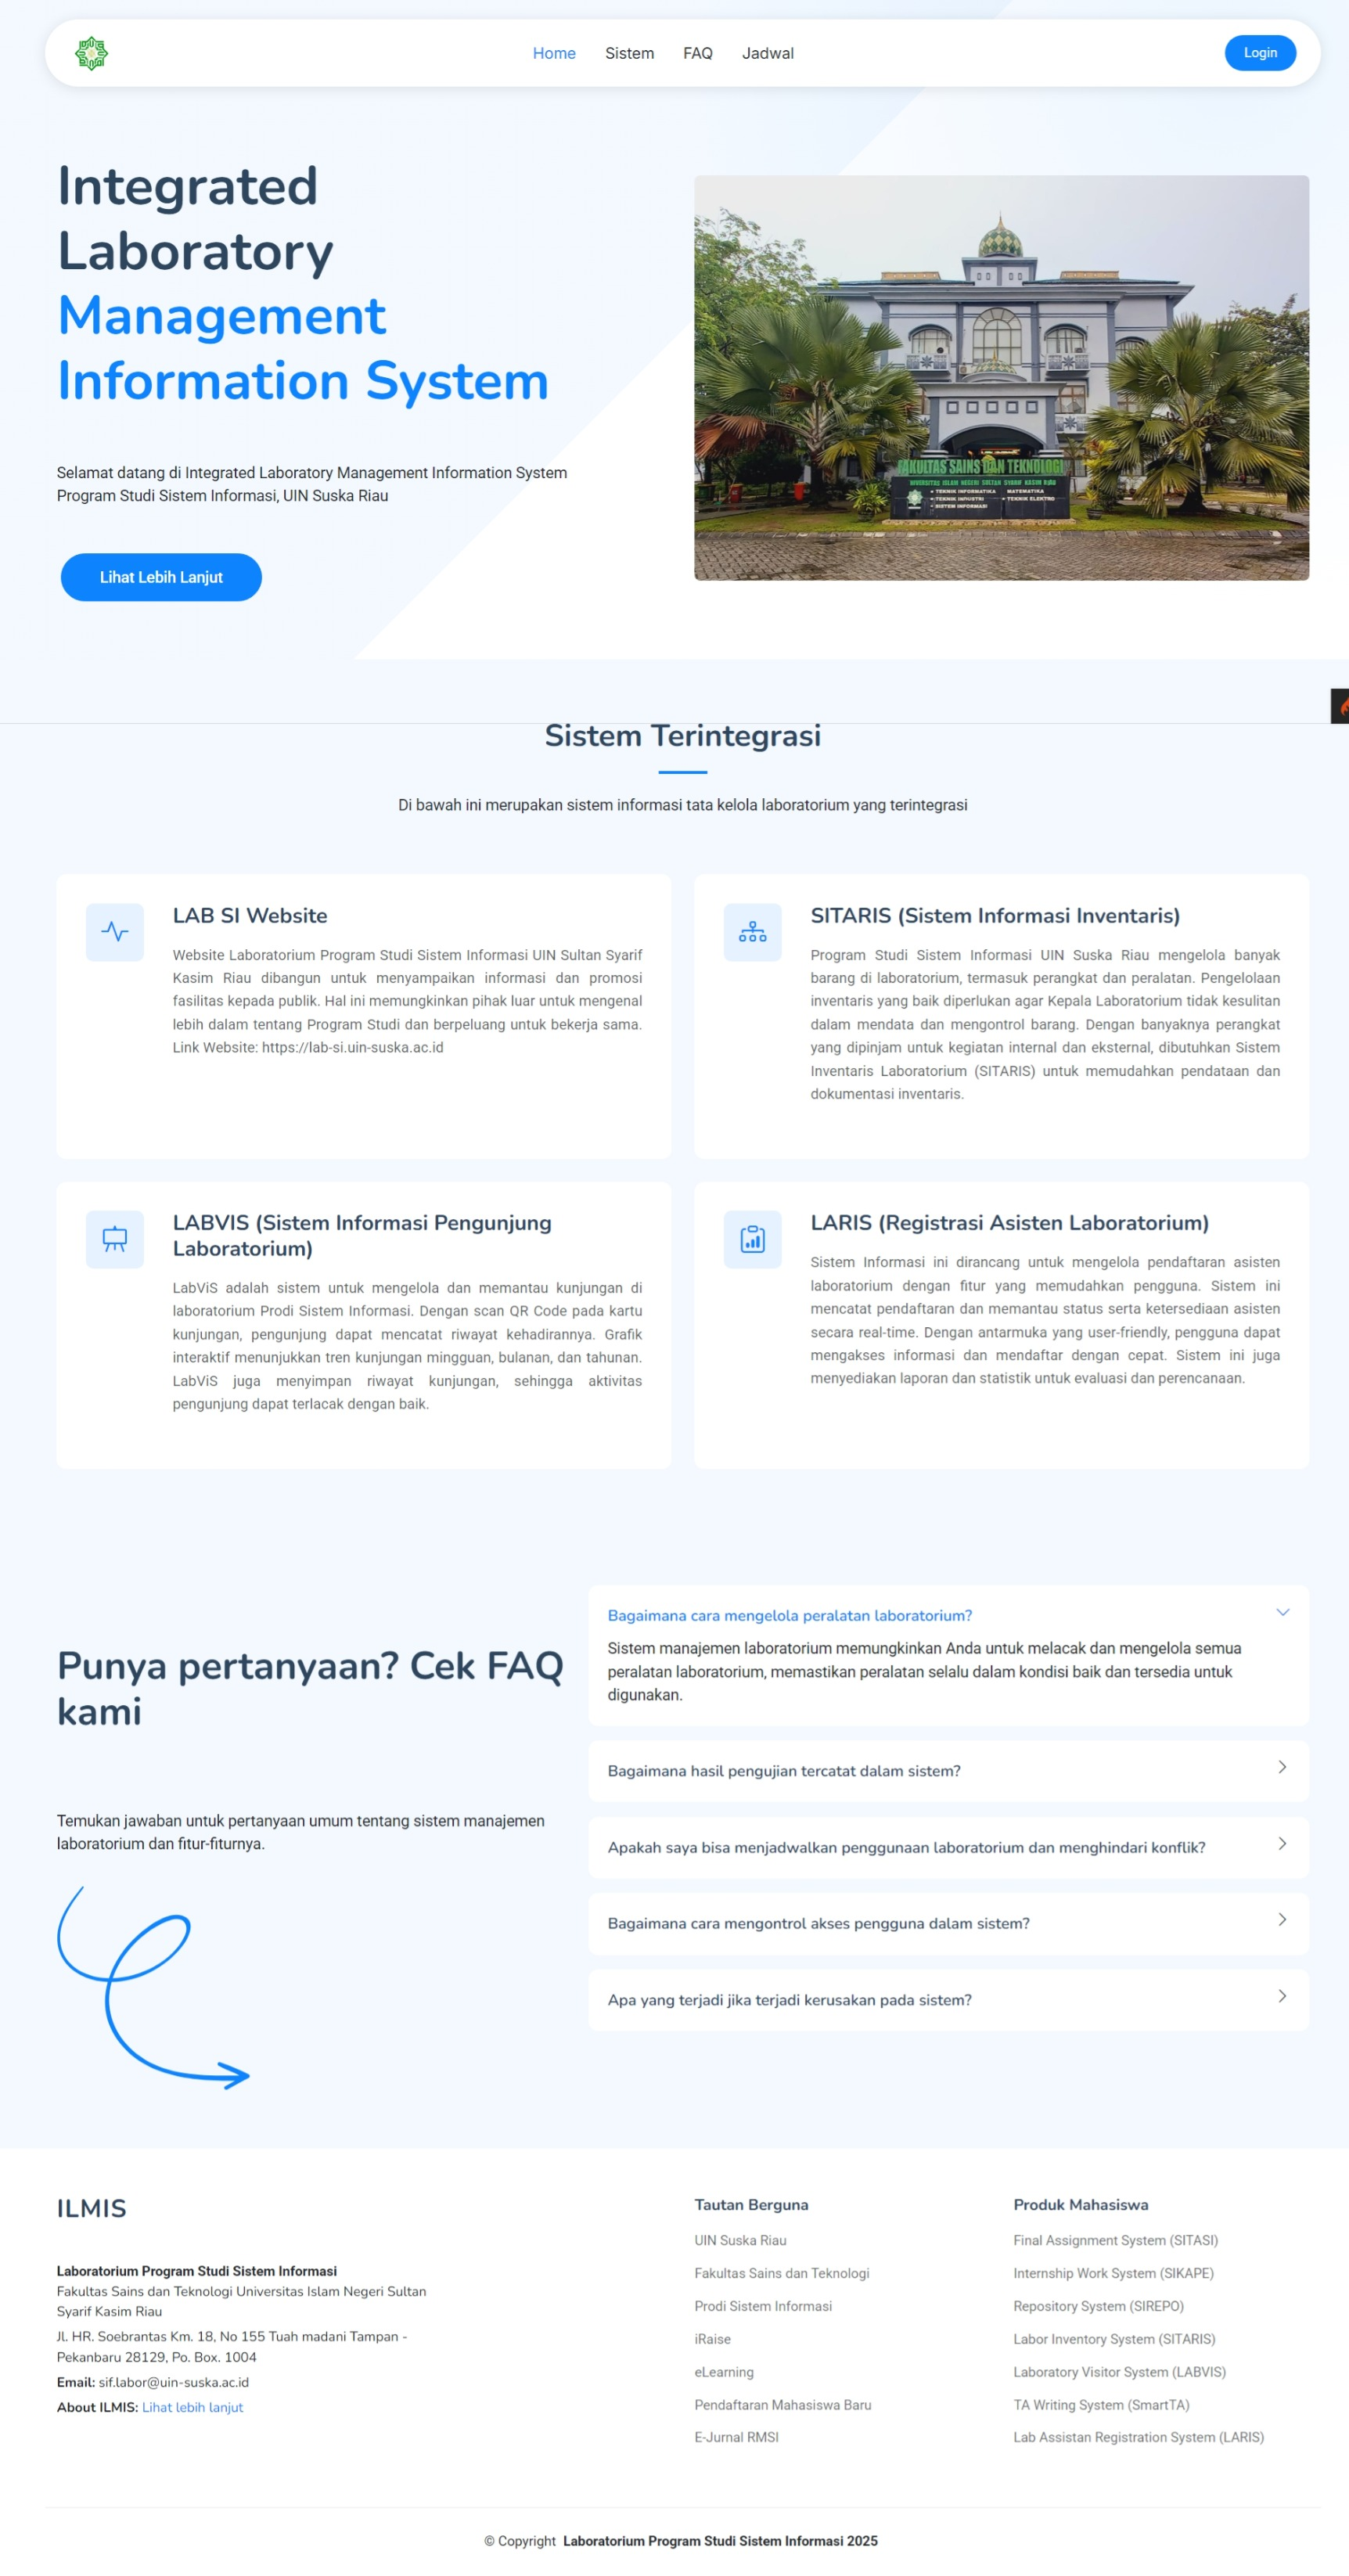
\includegraphics[width=0.82\textwidth]{konten/gambar/hasil/landing-page.jpeg}
	\caption{Tampilan \textit{Landing Page} ILMIS}
	\label{fig:landing-page}
\end{figure}

\begin{figure}
	\centering
	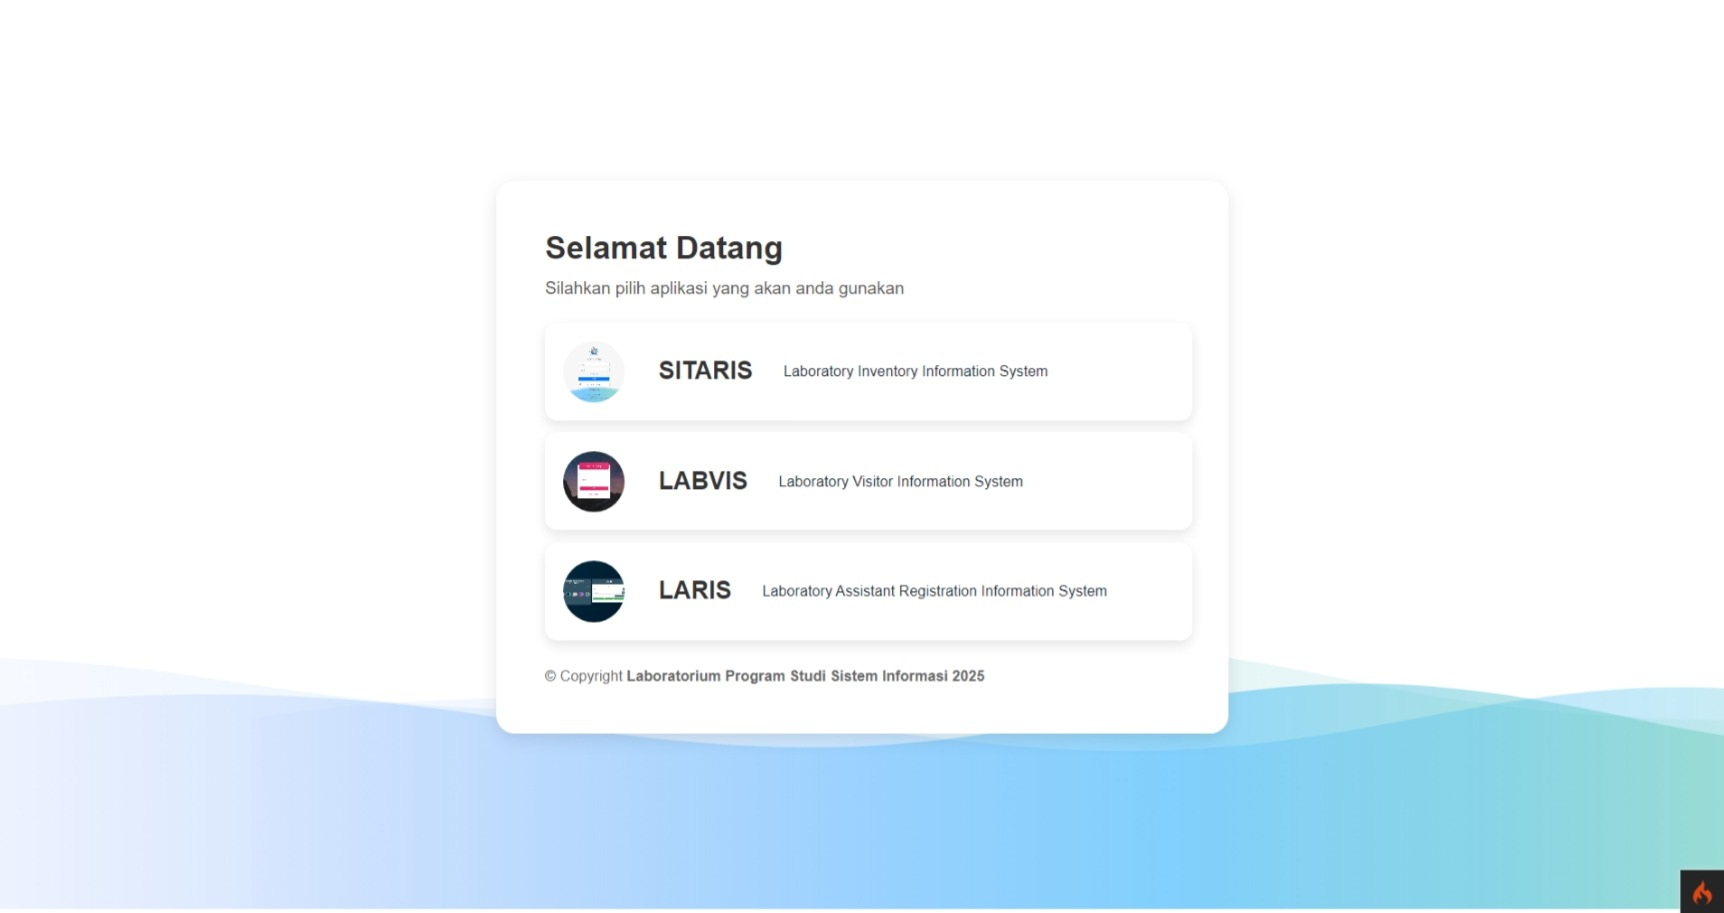
\includegraphics[width=0.82\textwidth]{konten/gambar/hasil/pilih-aplikasi.jpeg}
	\caption{Tampilan Pilihan Aplikasi untuk \textit{Login}}
	\label{fig:pilih-login}
\end{figure}

\begin{figure}
	\centering
	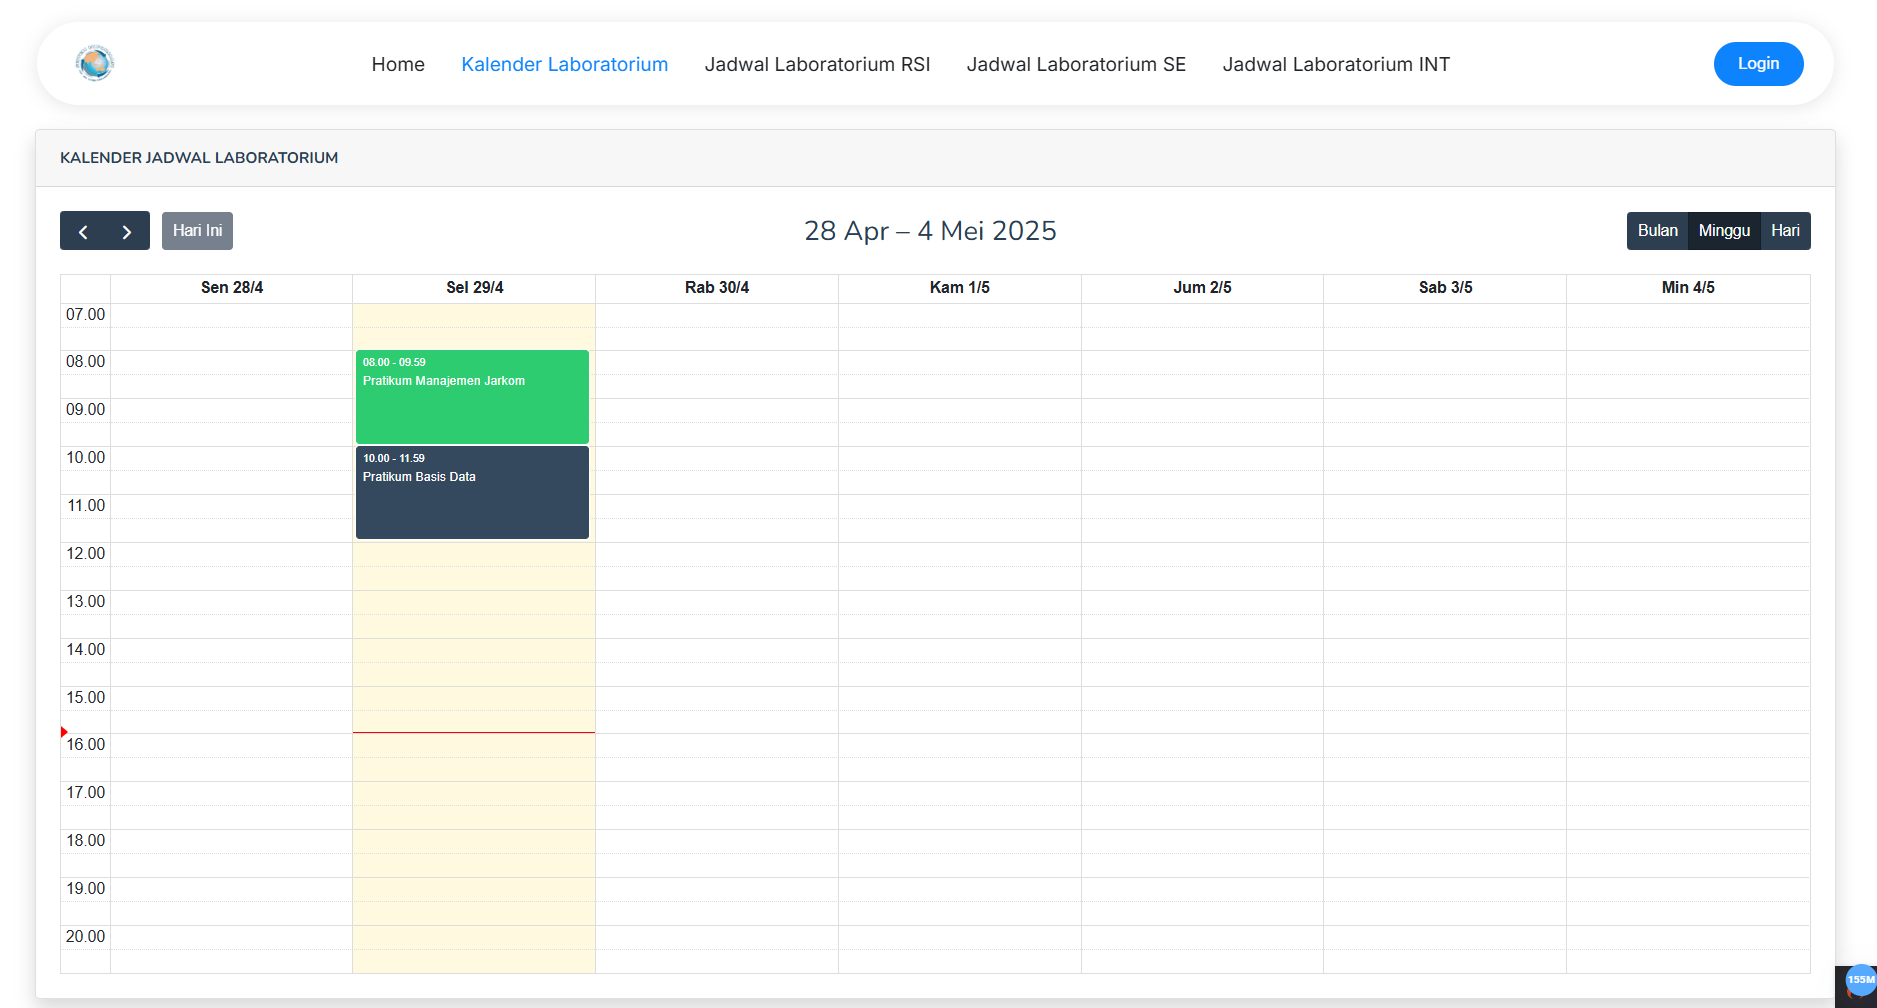
\includegraphics[width=0.82\textwidth]{konten/gambar/hasil/kalender.png}
	\caption{Tampilan Kalender ILMIS}
	\label{fig:kalender}
\end{figure}

\begin{figure}
	\centering
	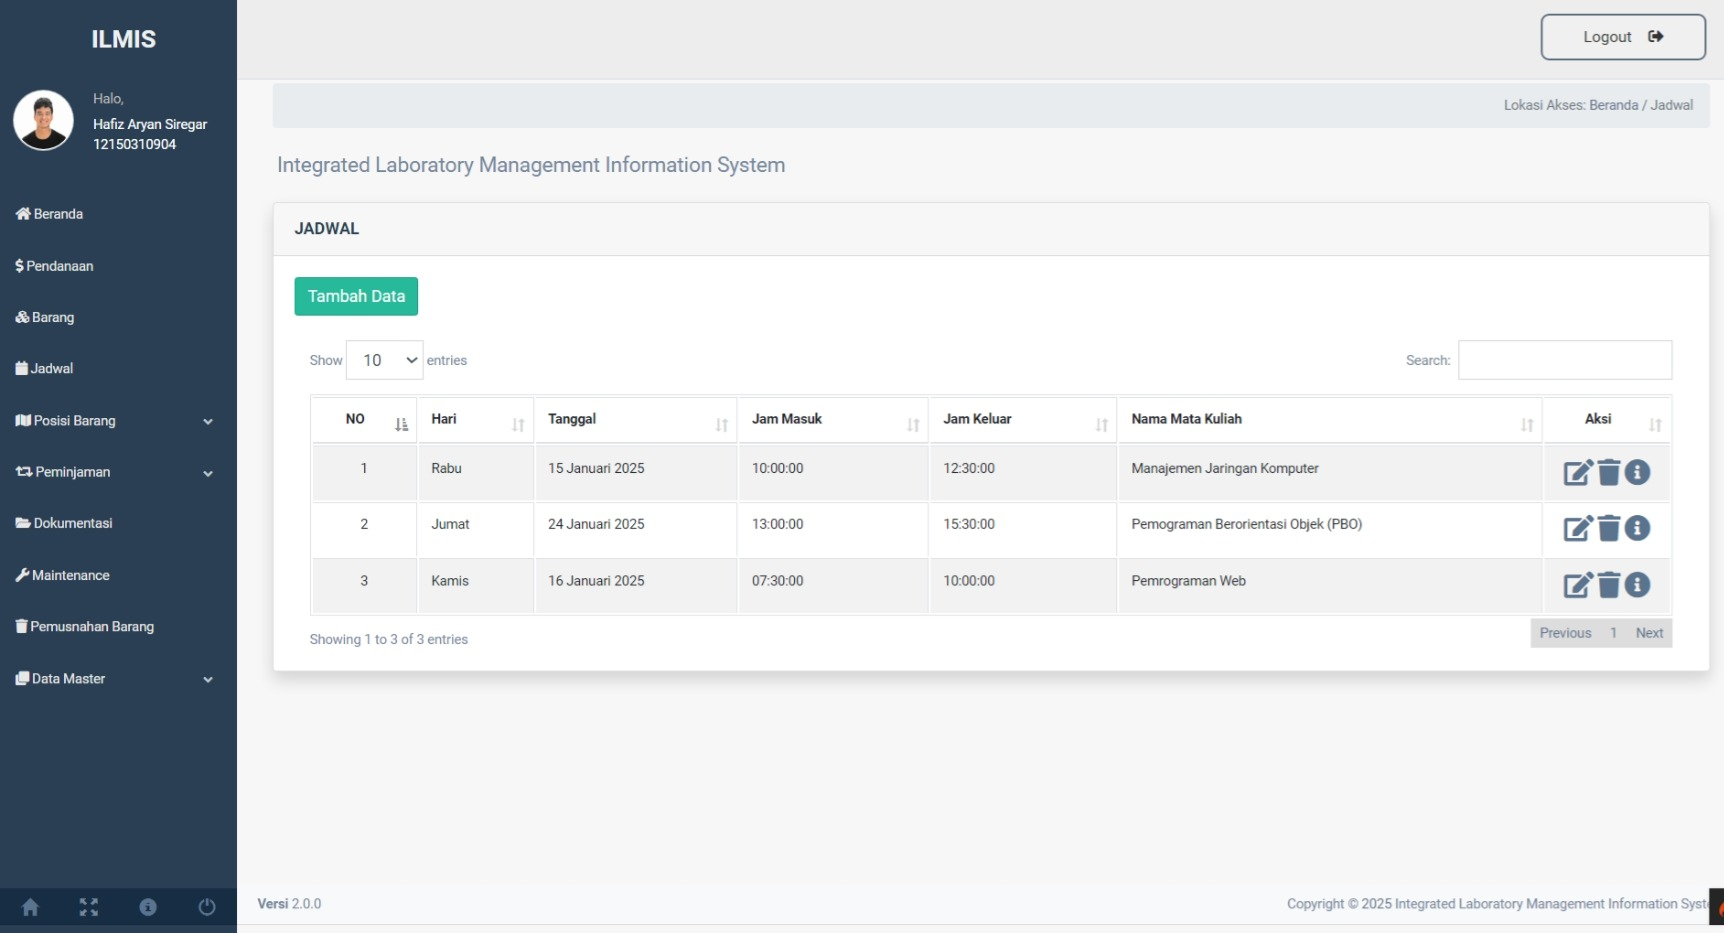
\includegraphics[width=0.82\textwidth]{konten/gambar/hasil/jadwal.jpeg}
	\caption{Tampilan Pengelolaan Jadwal Laboratorium}
	\label{fig:jadwal-keseluruhan}
\end{figure}
\begin{figure}
	\centering
	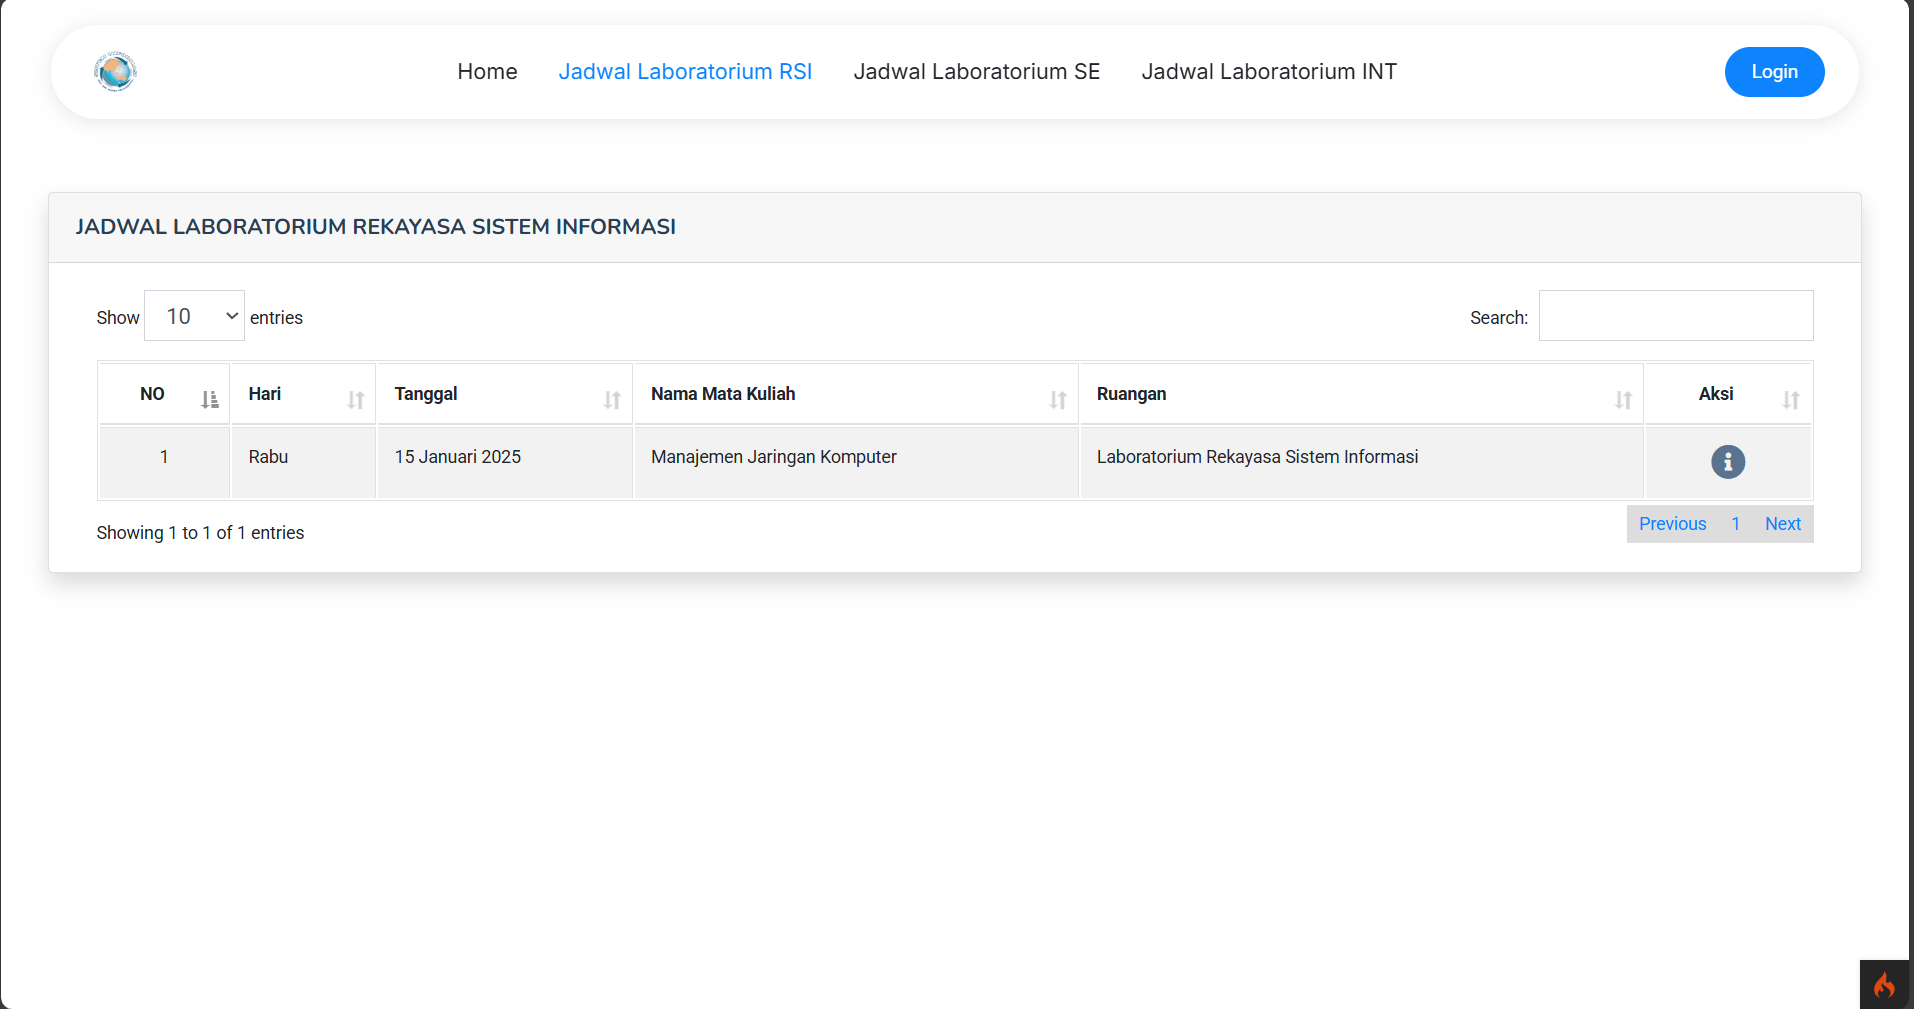
\includegraphics[width=0.82\textwidth]{konten/gambar/hasil/labor-rsi.png}
	\caption{Tampilan Pengelolaan Jadwal Laboratorium RSI}
	\label{fig:jadwal-rsi}
\end{figure}
\begin{figure}
	\centering
	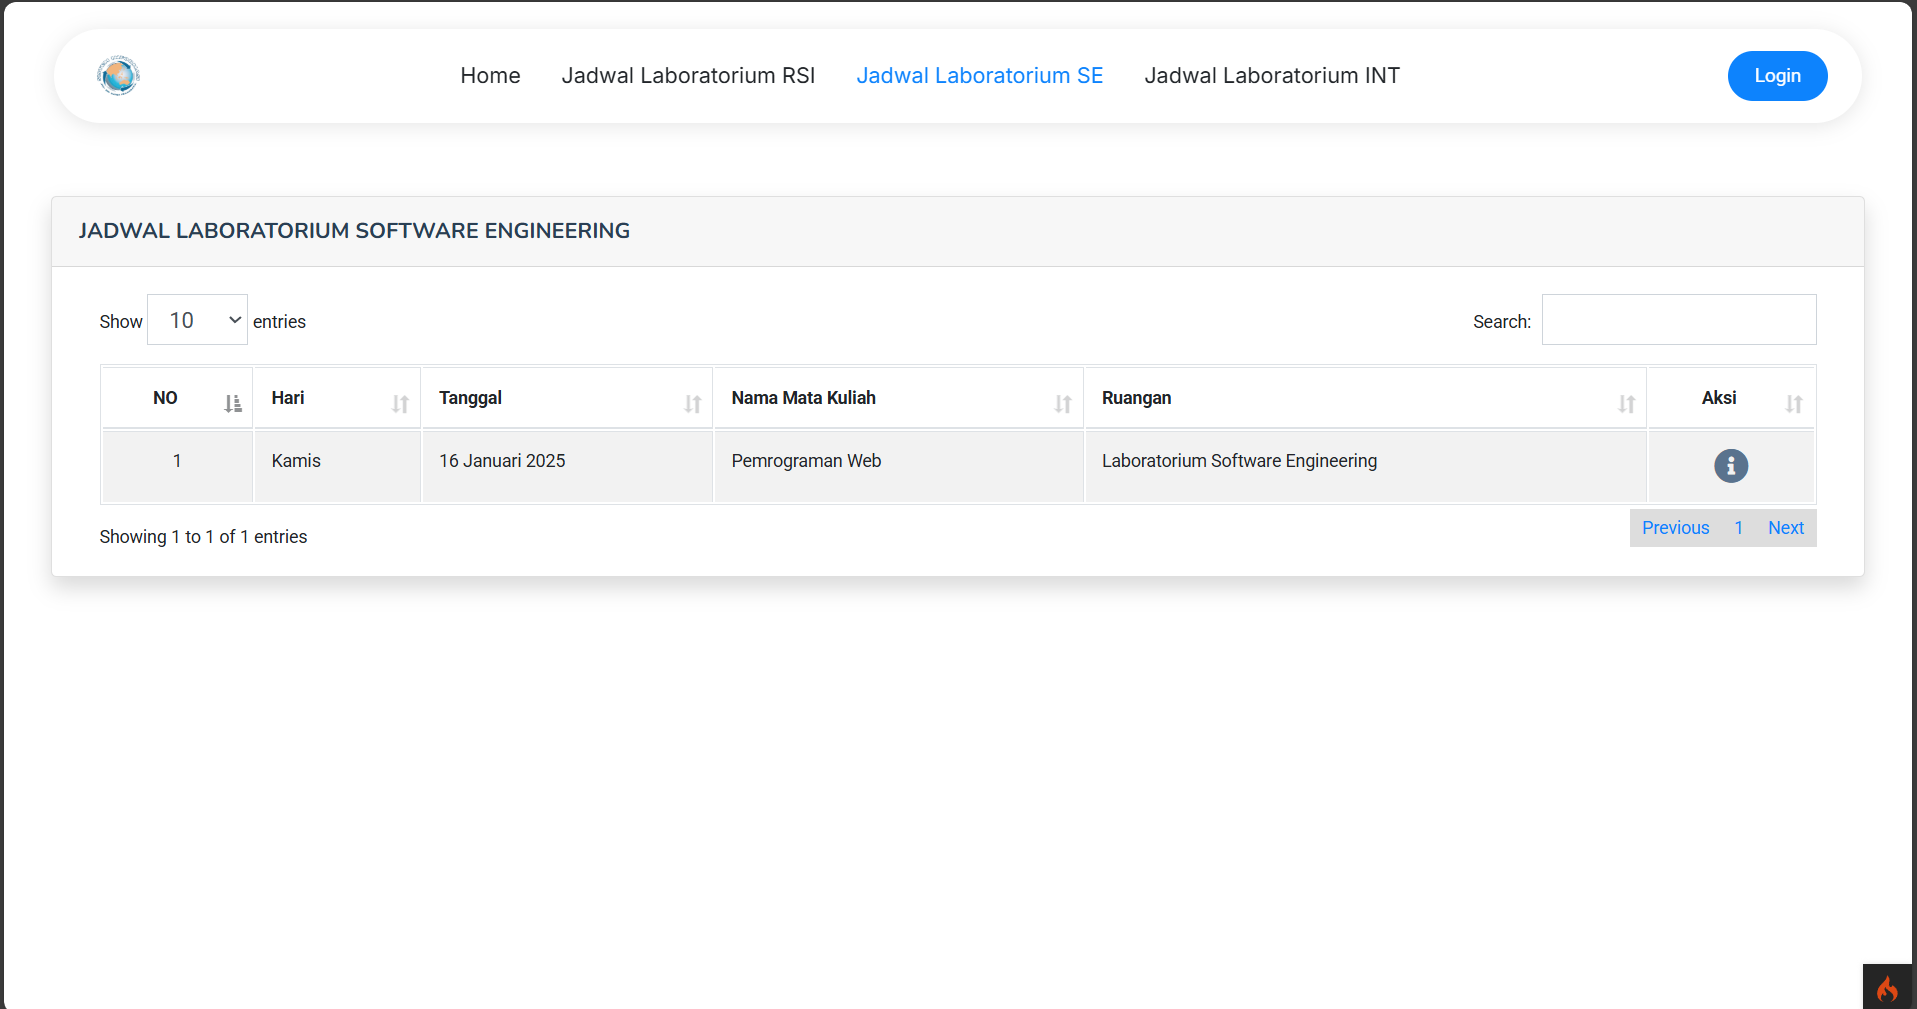
\includegraphics[width=0.82\textwidth]{konten/gambar/hasil/labor-se.png}
	\caption{Tampilan Pengelolaan Jadwal Laboratorium SE}
	\label{fig:jadwal-se}
\end{figure}
\begin{figure}
	\centering
	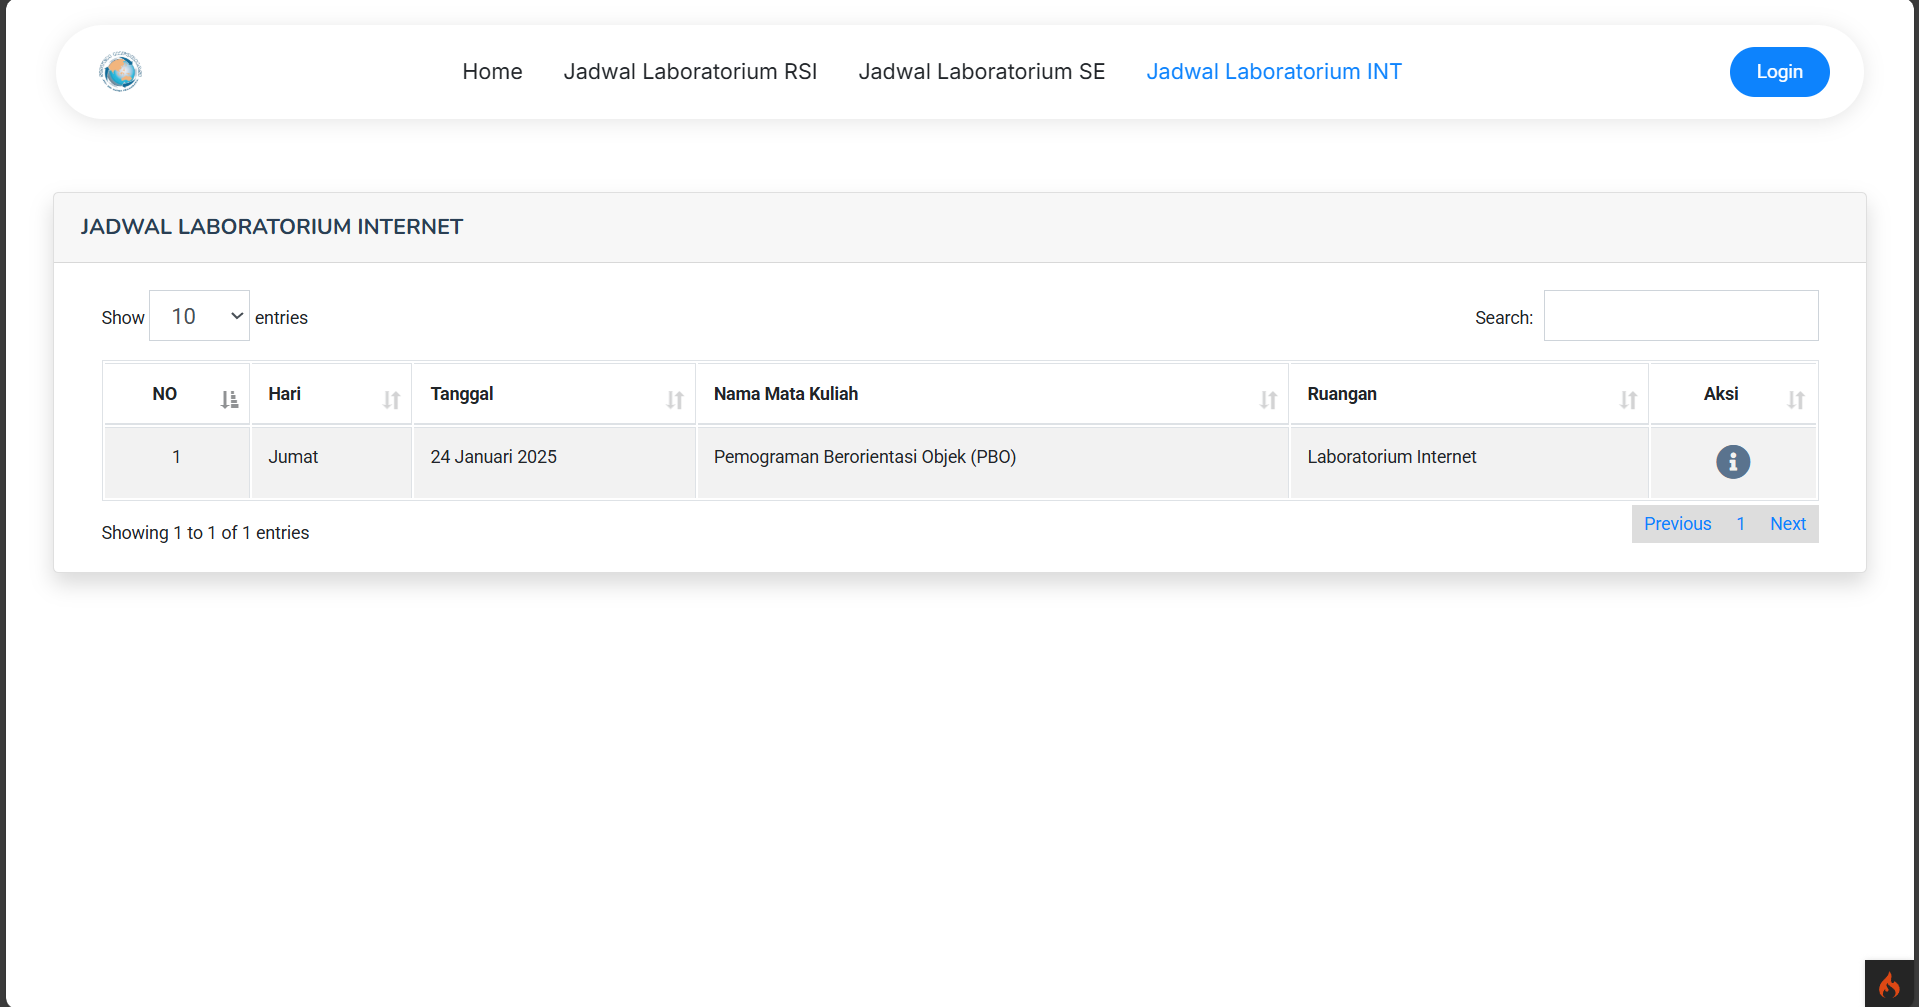
\includegraphics[width=0.82\textwidth]{konten/gambar/hasil/labor-int.png}
	\caption{Tampilan Pengelolaan Jadwal Laboratorium INT}
	\label{fig:jadwal-int}
\end{figure}

\begin{figure}
	\centering
	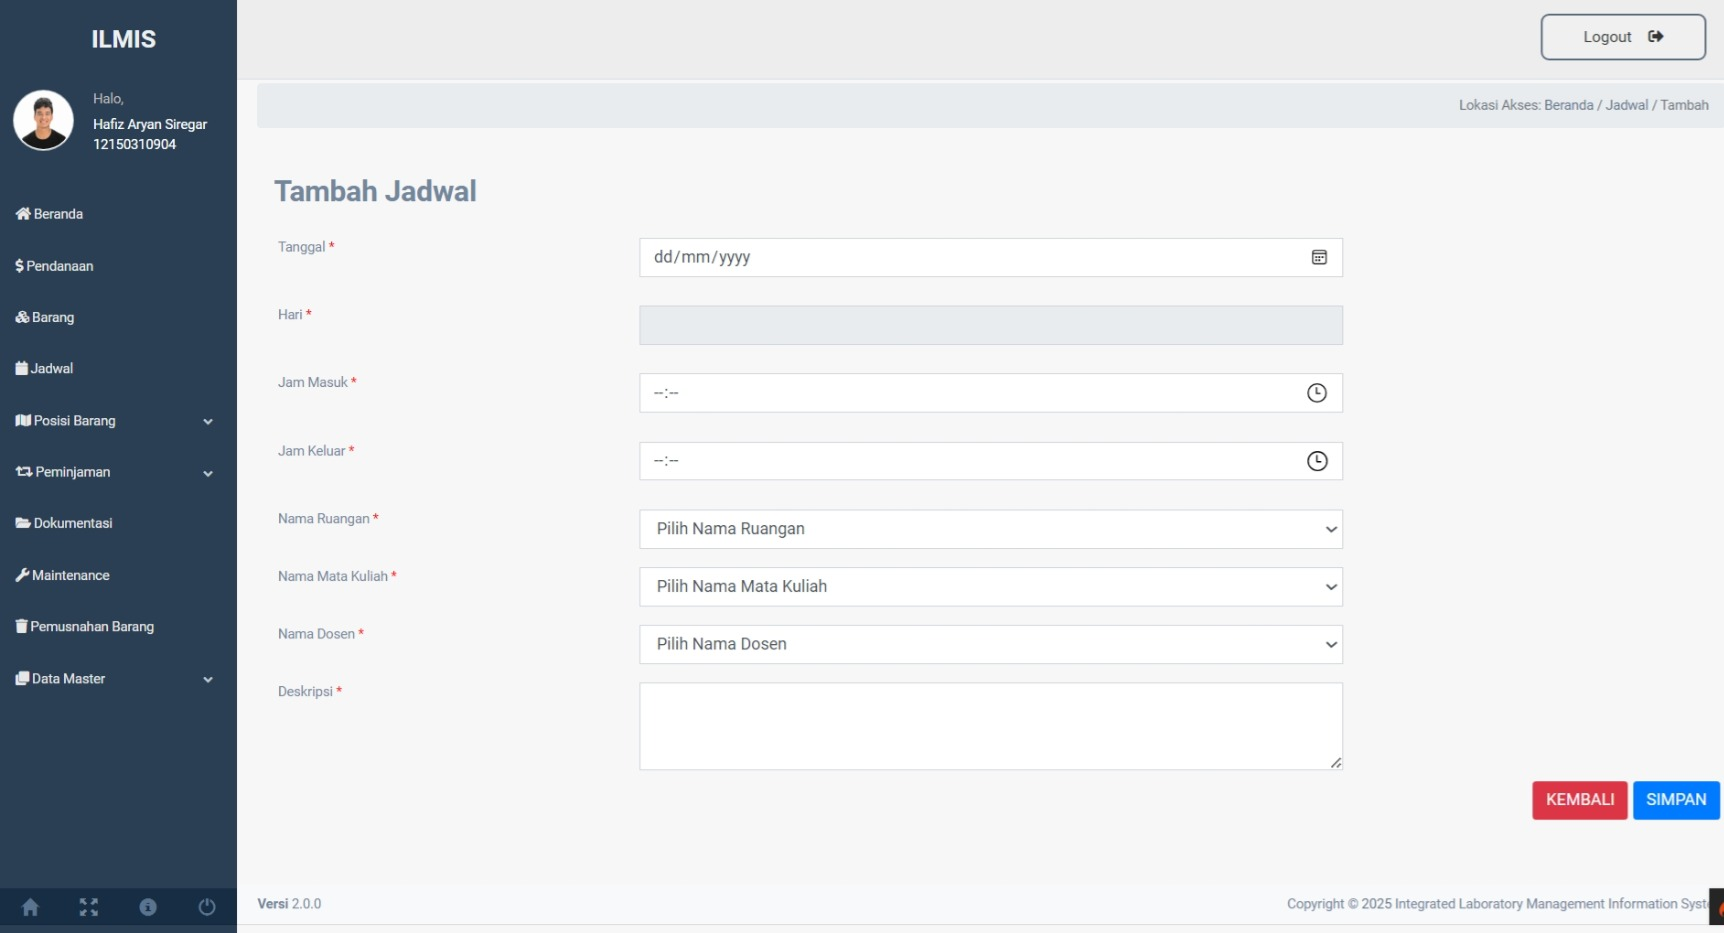
\includegraphics[width=0.82\textwidth]{konten/gambar/hasil/tambah-jadwal.jpeg}
	\caption{Tampilan Tambah Jadwal Laboratorium}
	\label{fig:tambah-jadwal}
\end{figure}

\begin{figure}
	\centering
	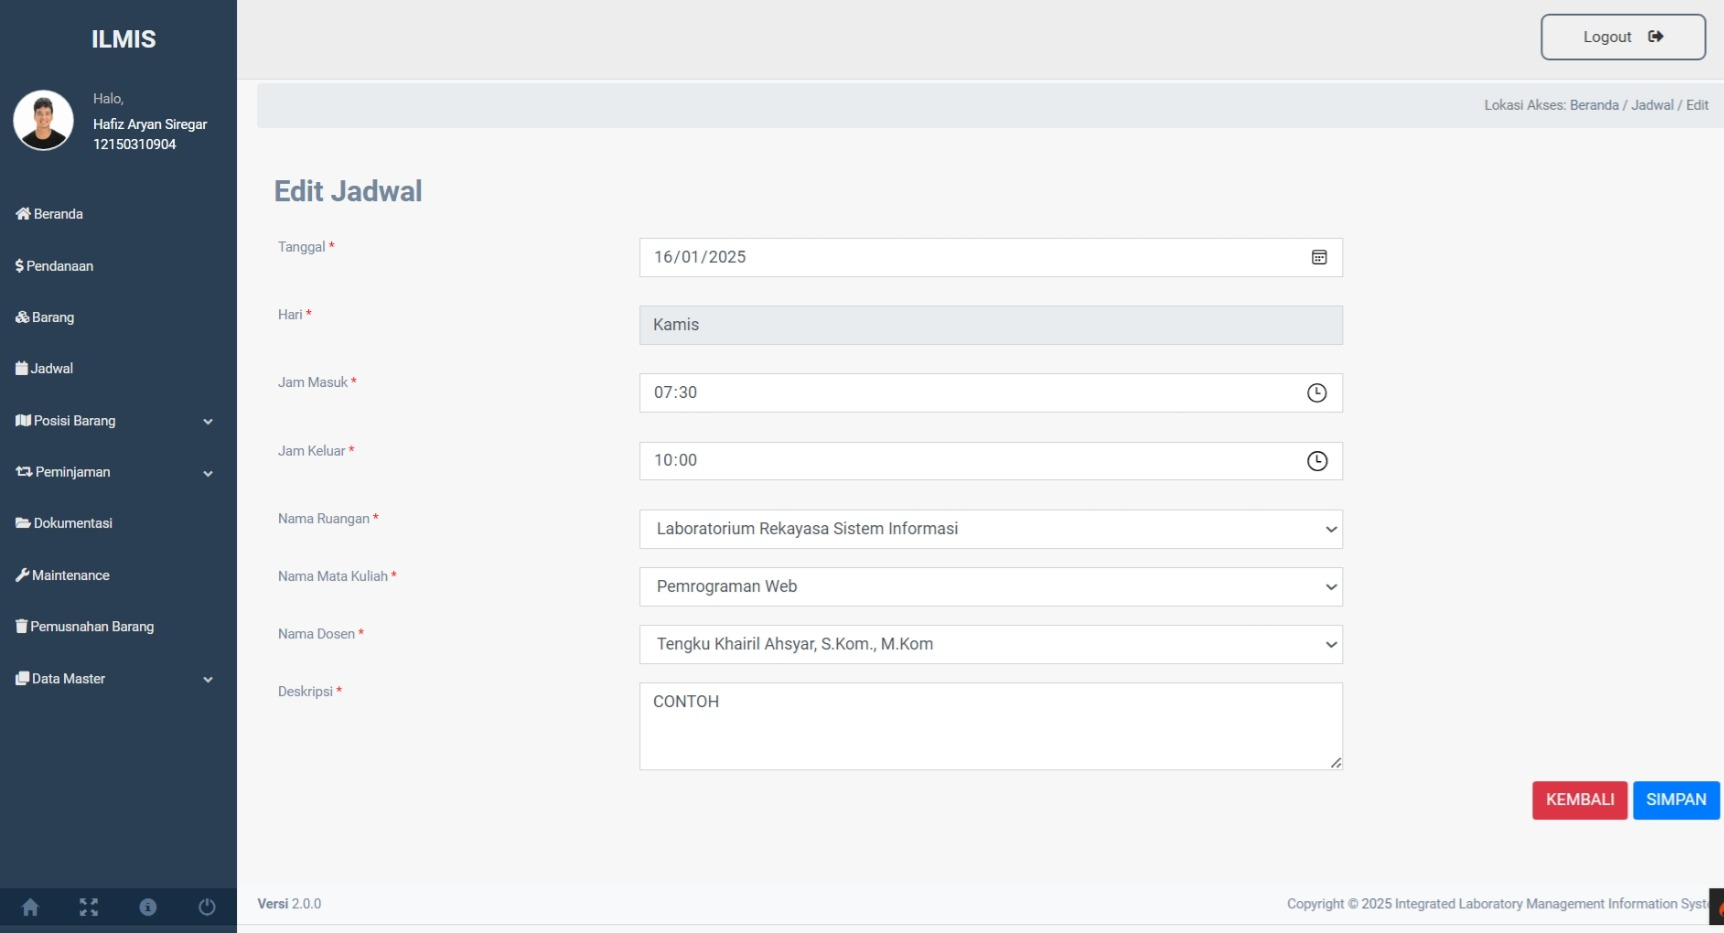
\includegraphics[width=0.82\textwidth]{konten/gambar/hasil/edit-jadwal.jpeg}
	\caption{Tampilan Edit Jadwal Laboratorium}
	\label{fig:edit-jadwal}
\end{figure}

\begin{figure}
	\centering
	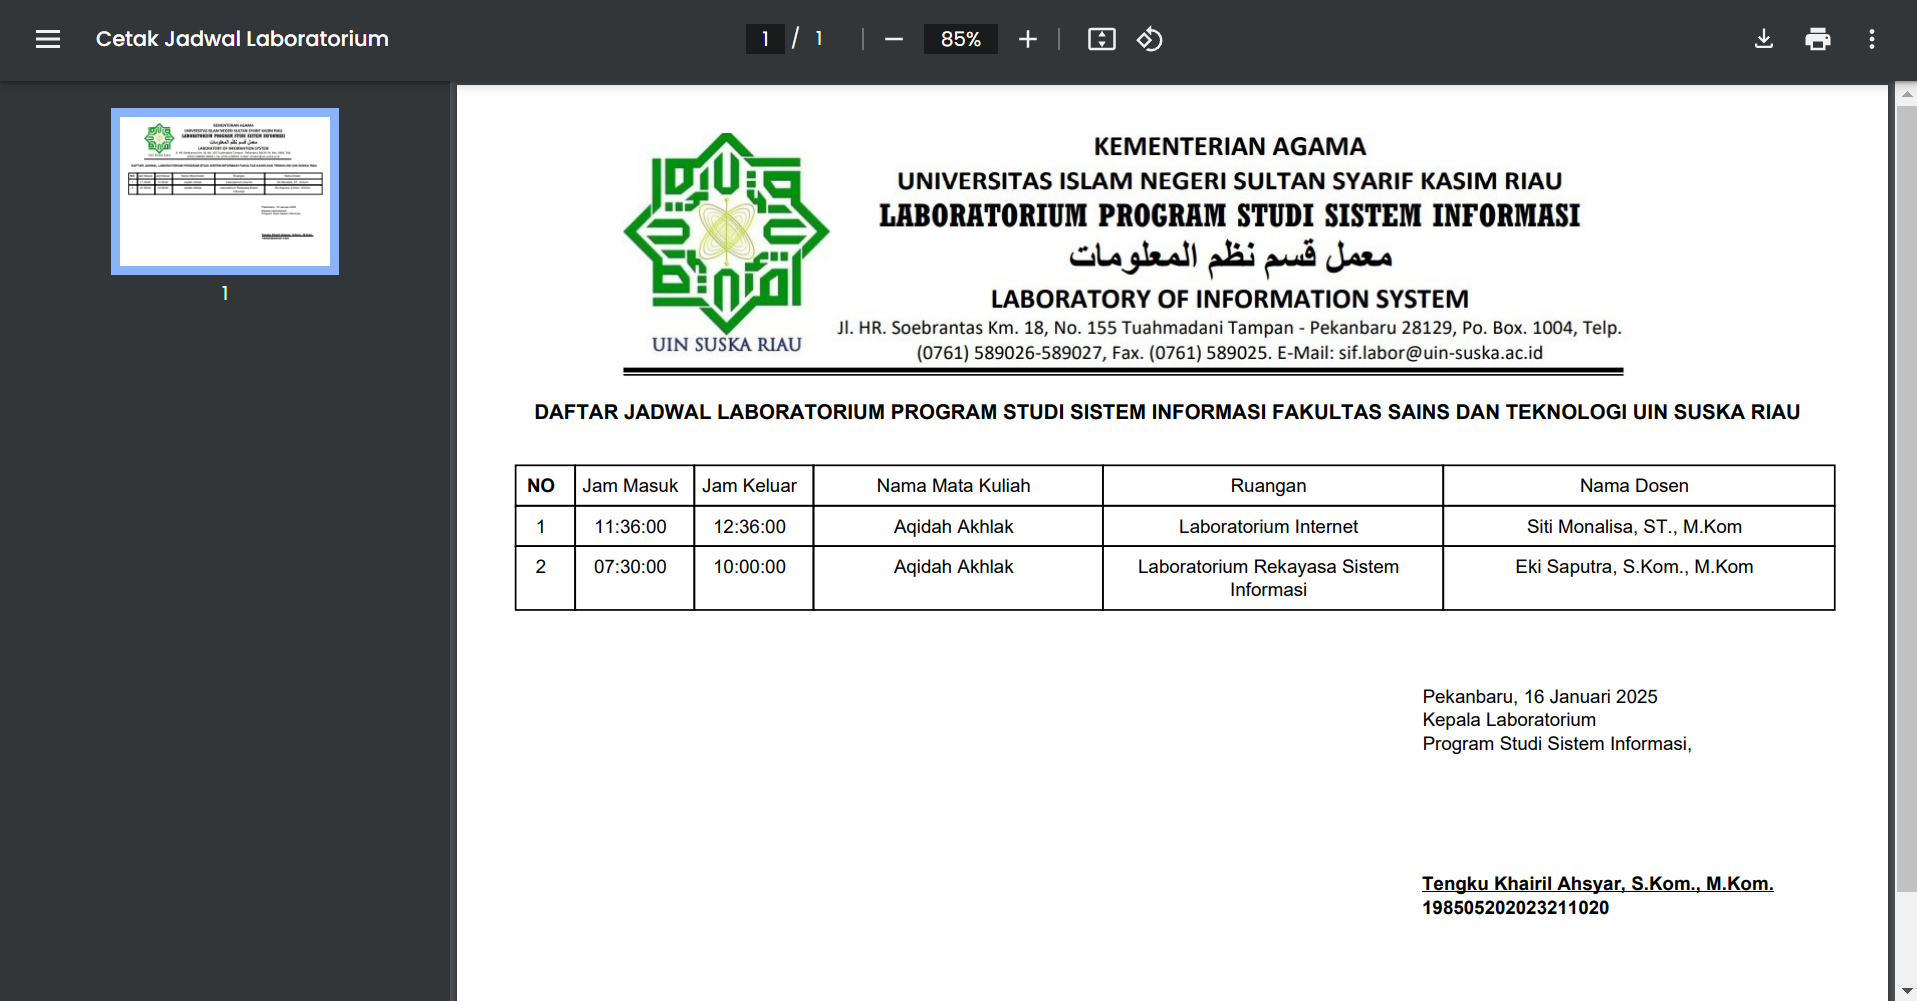
\includegraphics[width=0.82\textwidth]{konten/gambar/hasil/cetak-jadwal.png}
	\caption{Tampilan Cetak Jadwal Laboratorium dalam Format PDF}
	\label{fig:cetak-jadwal}
\end{figure}

\begin{figure}
	\centering
	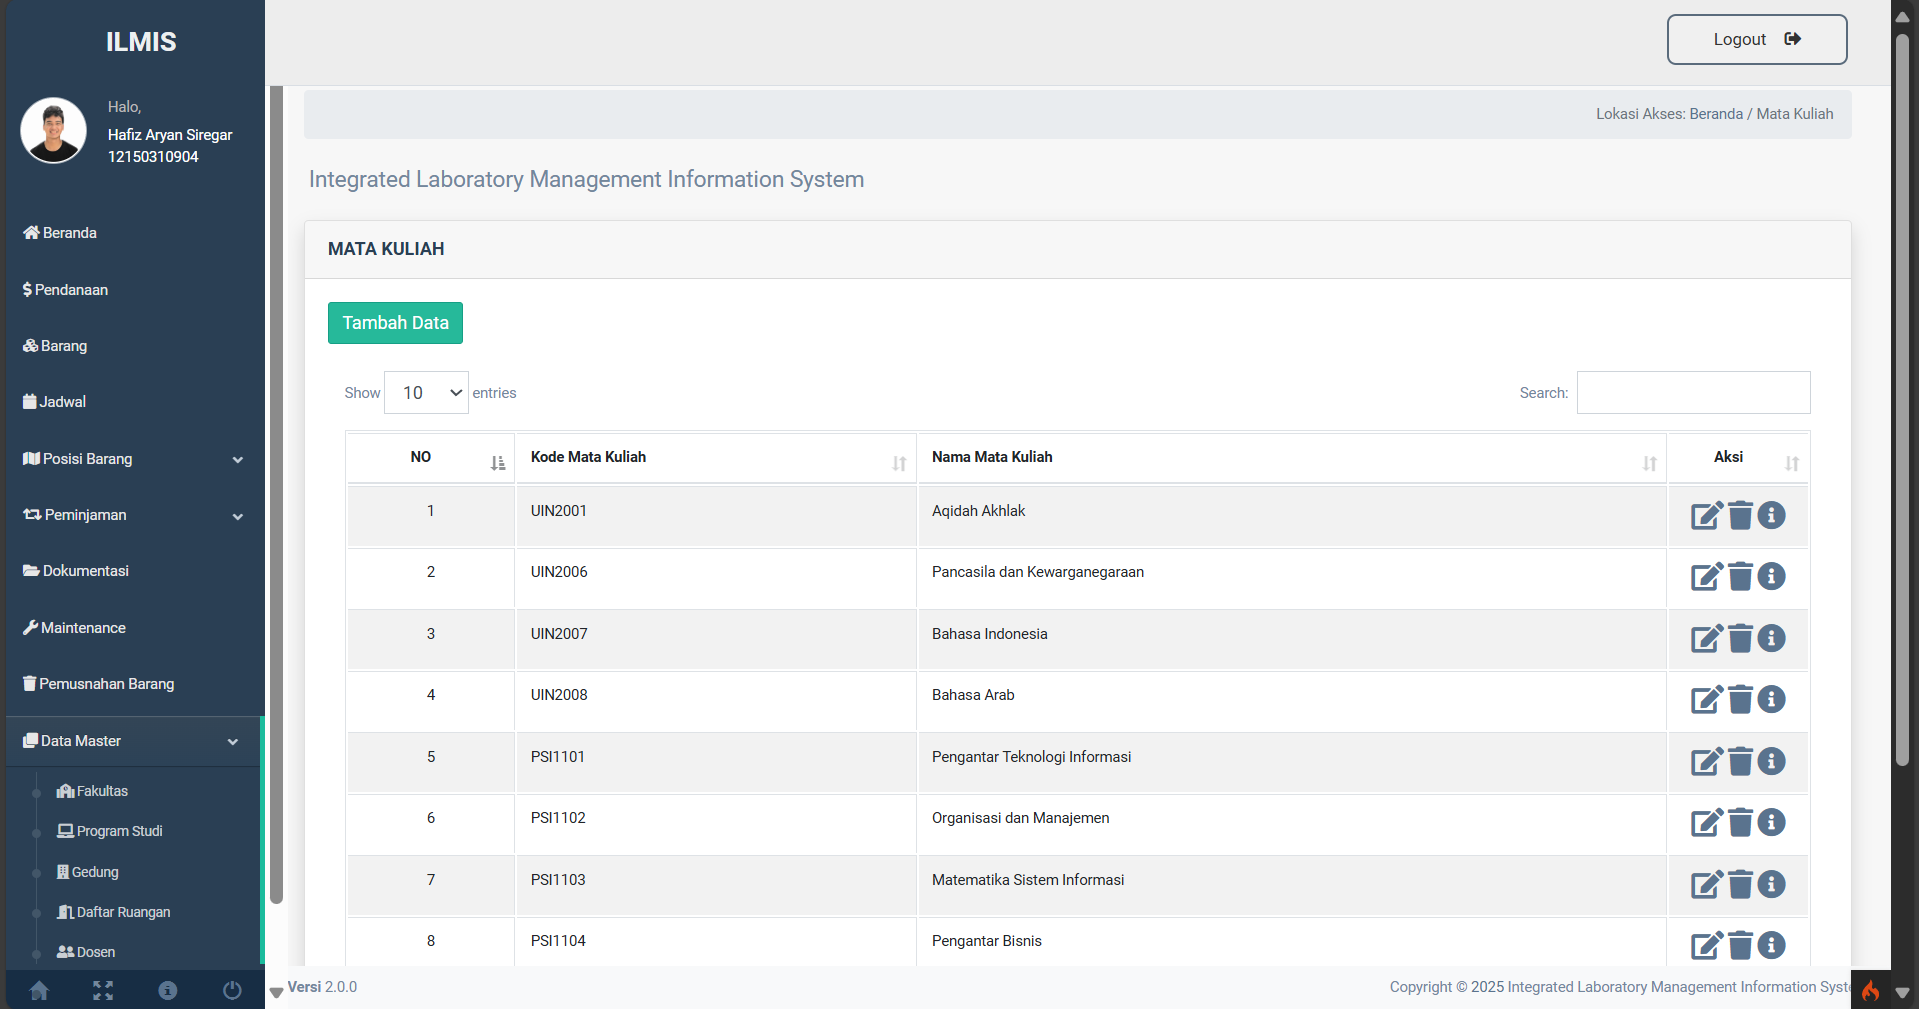
\includegraphics[width=0.82\textwidth]{konten/gambar/hasil/matkul.png}
	\caption{Tampilan Kelola Mata Kuliah Laboratorium}
	\label{fig:matkul}
\end{figure}

\begin{figure}
	\centering
	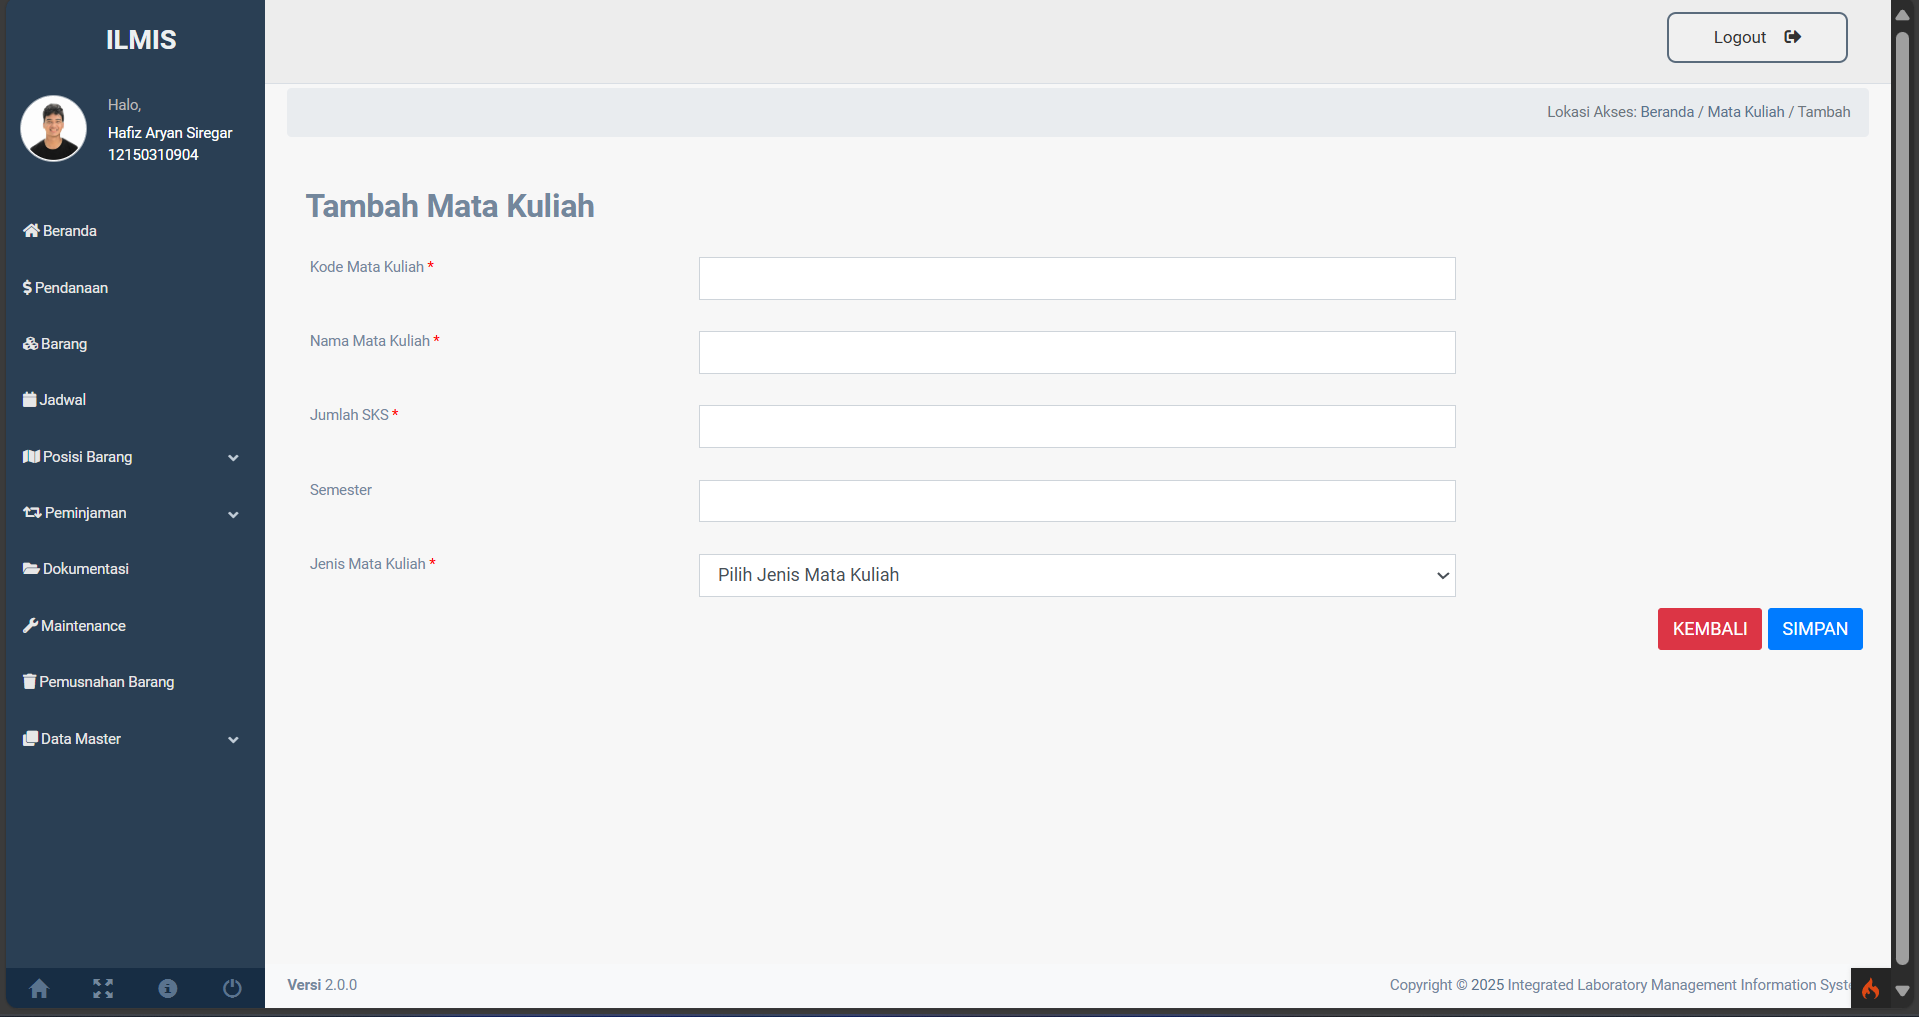
\includegraphics[width=0.82\textwidth]{konten/gambar/hasil/tambah-matkul.png}
	\caption{Tampilan Tambah Mata Kuliah Laboratorium}
	\label{fig:tambah-matkul}
\end{figure}

\begin{figure}
	\centering
	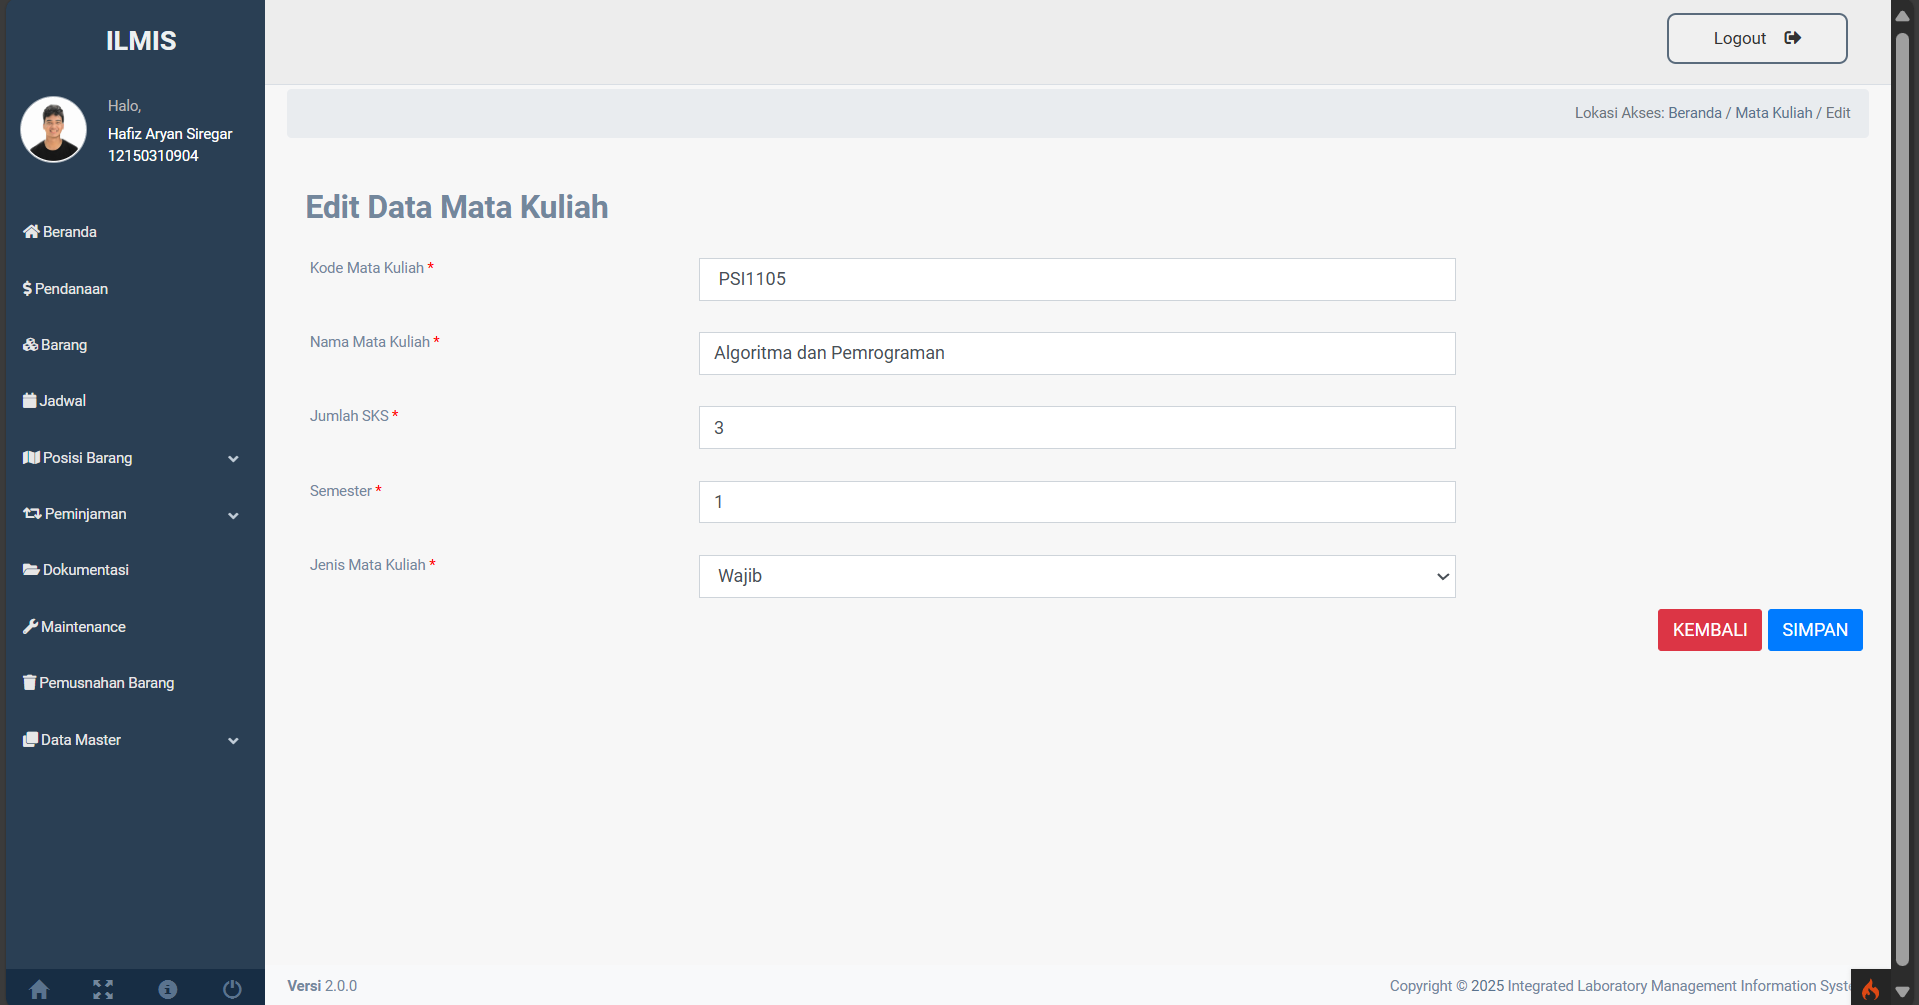
\includegraphics[width=0.82\textwidth]{konten/gambar/hasil/edit-matkul.png}
	\caption{Tampilan Edit Mata Kuliah Laboratorium}
	\label{fig:edit-matkul}
\end{figure}

\begin{figure}
	\centering
	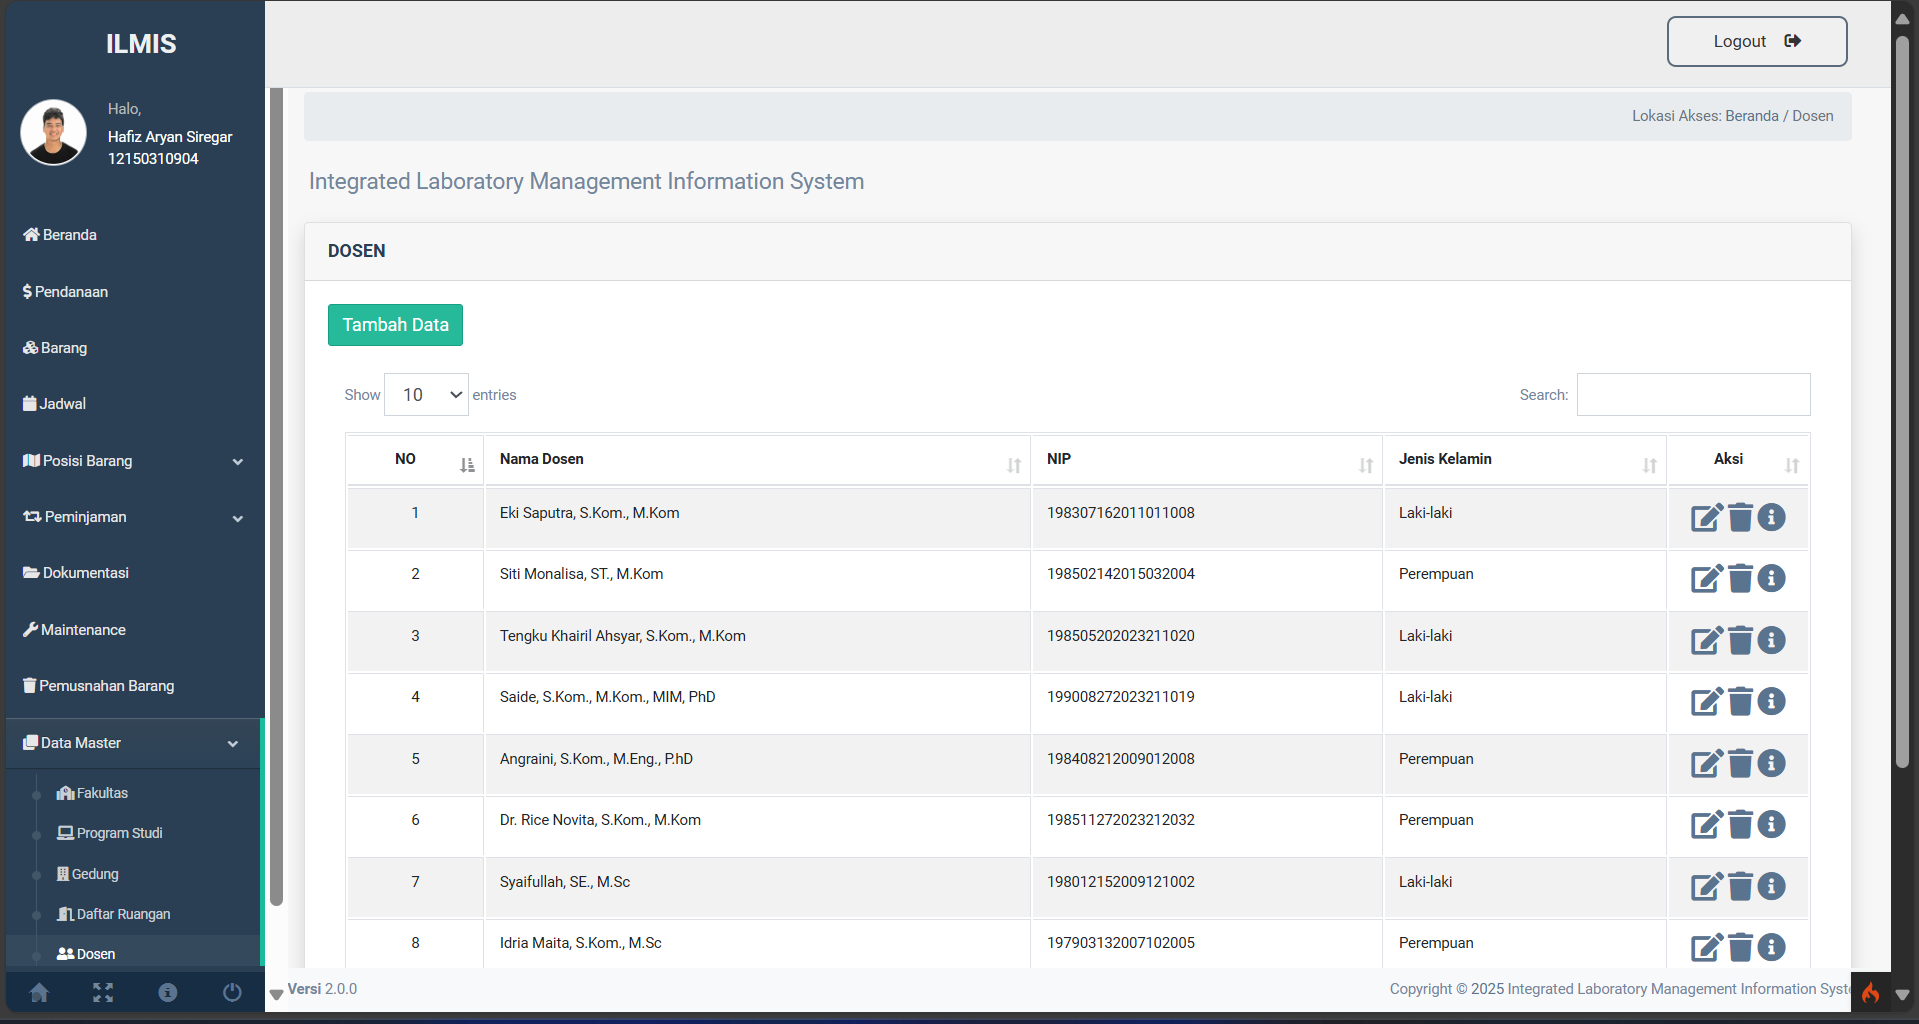
\includegraphics[width=0.82\textwidth]{konten/gambar/hasil/dosen.png}
	\caption{Tampilan Kelola Dosen Laboratorium}
	\label{fig:dosen}
\end{figure}

\begin{figure}
	\centering
	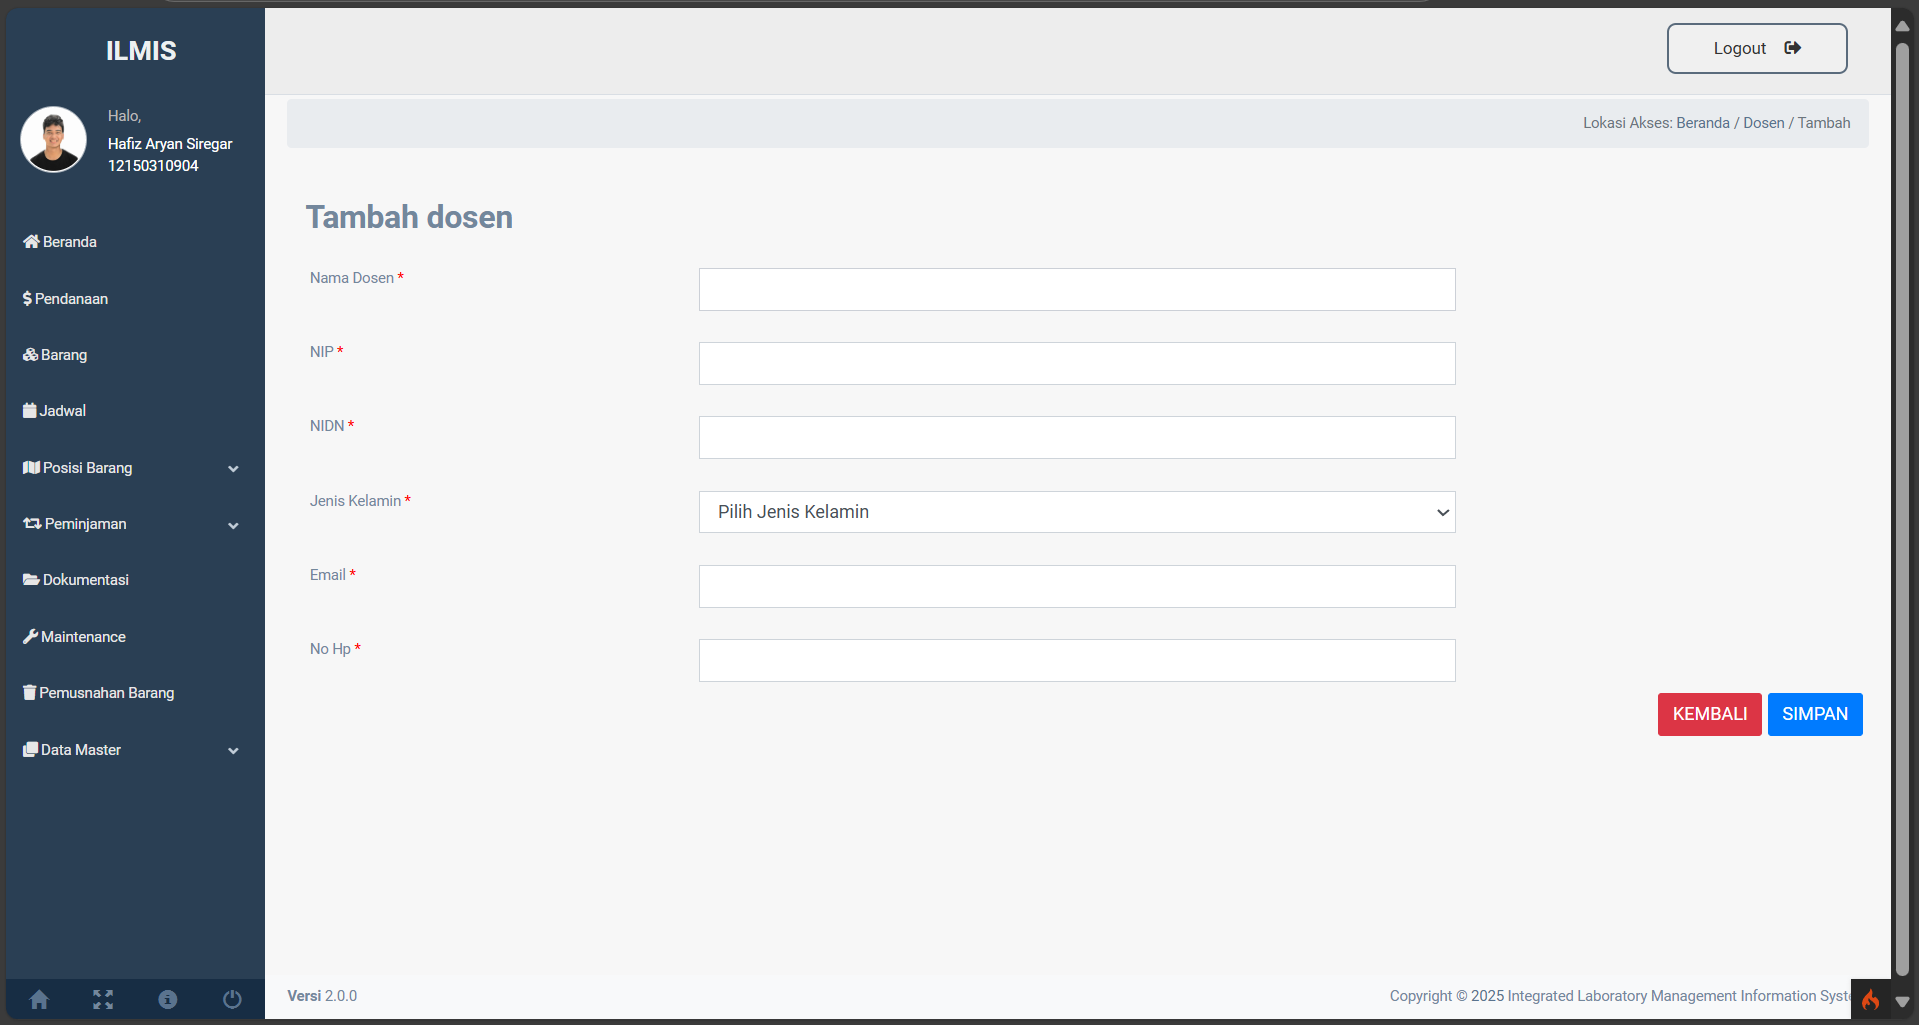
\includegraphics[width=0.82\textwidth]{konten/gambar/hasil/tambah-dosen.png}
	\caption{Tampilan Tambah Dosen Laboratorium}
	\label{fig:tambah-dosen}
\end{figure}

\begin{figure}
	\centering
	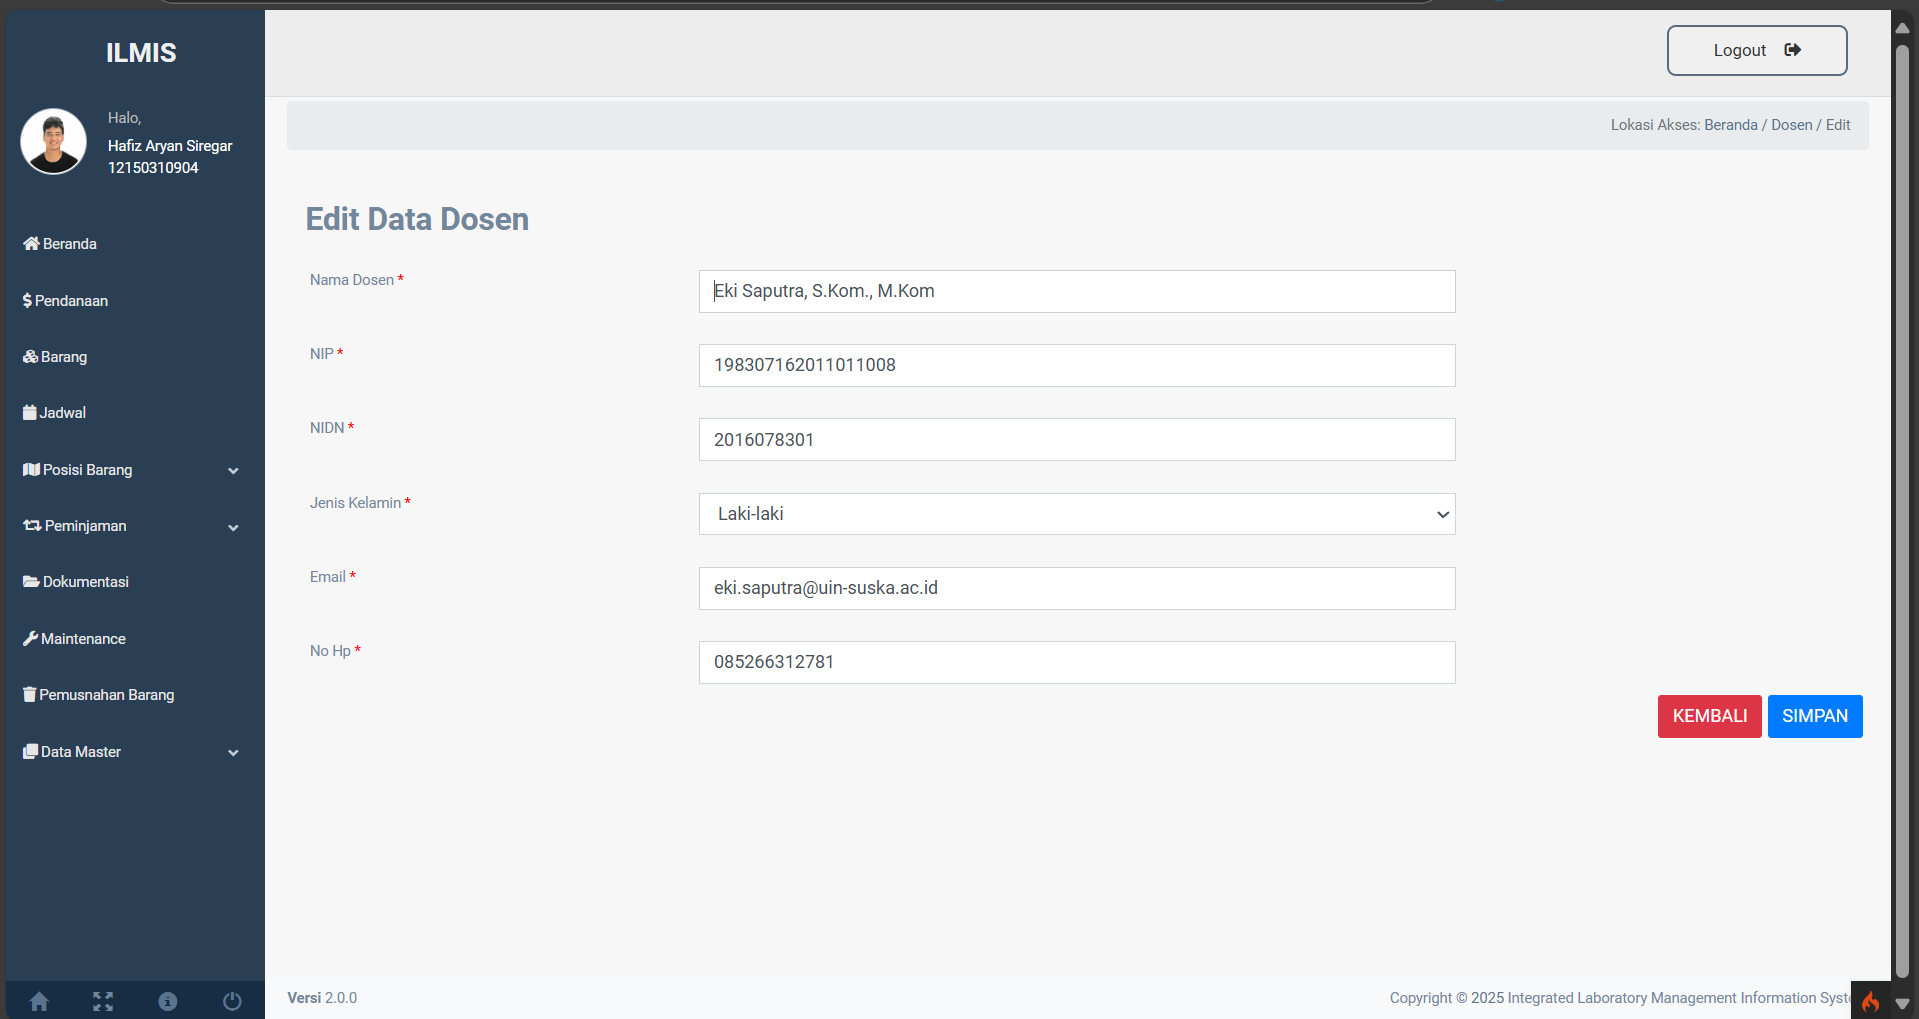
\includegraphics[width=0.82\textwidth]{konten/gambar/hasil/edit-dosen.png}
	\caption{Tampilan Edit Dosen Laboratorium}
	\label{fig:edit-dosen}
\end{figure}

\begin{figure}
	\centering
	\includegraphics[width=0.82\linewidth]{konten/gambar/source-code.png}
	\caption{\textit{Source Code}}
	\label{fig:source-code}
\end{figure}